\documentclass{article}
\PassOptionsToPackage{numbers,sort&compress}{natbib}
\usepackage[eandd]{neurips_2026}
\usepackage[utf8]{inputenc}
\usepackage[T1]{fontenc}
\usepackage{amsmath,amsfonts,booktabs,graphicx,microtype,xcolor,url,tabularx,array,float,flafter}
\usepackage{hyperref}
\hypersetup{hidelinks}
% Generated from claim_ledger.tsv; do not edit by hand.
\providecommand{\claimvalue}[1]{%
  \ifcsname OAEClaim#1\endcsname%
    \csname OAEClaim#1\endcsname%
  \else%
    \PackageError{openaffect-claims}{Unknown claim #1}%
      {Rebuild manuscript assets from the frozen claim ledger.}%
  \fi%
}
\expandafter\def\csname OAEClaimC01\endcsname{0.627}% \claimvalue{C01}
\expandafter\def\csname OAEClaimC02\endcsname{0.3739}% \claimvalue{C02}
\expandafter\def\csname OAEClaimC03\endcsname{0.4464}% \claimvalue{C03}
\expandafter\def\csname OAEClaimC04\endcsname{0.0706}% \claimvalue{C04}
\expandafter\def\csname OAEClaimC05\endcsname{0.0396}% \claimvalue{C05}
\expandafter\def\csname OAEClaimC06\endcsname{0.1143}% \claimvalue{C06}
\expandafter\def\csname OAEClaimC07\endcsname{0.0015}% \claimvalue{C07}
\expandafter\def\csname OAEClaimC08\endcsname{-0.0008}% \claimvalue{C08}
\expandafter\def\csname OAEClaimC09\endcsname{0.9642}% \claimvalue{C09}
\expandafter\def\csname OAEClaimC10\endcsname{0.1733}% \claimvalue{C10}
\expandafter\def\csname OAEClaimC11\endcsname{0.8987}% \claimvalue{C11}
\expandafter\def\csname OAEClaimC12\endcsname{0.0234}% \claimvalue{C12}
\expandafter\def\csname OAEClaimC13\endcsname{0.1989}% \claimvalue{C13}
\expandafter\def\csname OAEClaimC14\endcsname{0.0126}% \claimvalue{C14}
\expandafter\def\csname OAEClaimC15\endcsname{0.4976}% \claimvalue{C15}
\expandafter\def\csname OAEClaimC16\endcsname{0.0133}% \claimvalue{C16}
\expandafter\def\csname OAEClaimC17\endcsname{0.3765}% \claimvalue{C17}
\expandafter\def\csname OAEClaimC18\endcsname{0.5405}% \claimvalue{C18}
\expandafter\def\csname OAEClaimC19\endcsname{0.3927}% \claimvalue{C19}
\expandafter\def\csname OAEClaimC20\endcsname{0.3776}% \claimvalue{C20}
\expandafter\def\csname OAEClaimC21\endcsname{0.0319}% \claimvalue{C21}
\expandafter\def\csname OAEClaimC22\endcsname{0.3422}% \claimvalue{C22}
\expandafter\def\csname OAEClaimC23\endcsname{0.2486}% \claimvalue{C23}
\expandafter\def\csname OAEClaimC24\endcsname{0.1676}% \claimvalue{C24}
\expandafter\def\csname OAEClaimC25\endcsname{0.1667}% \claimvalue{C25}
\expandafter\def\csname OAEClaimC26\endcsname{0.2134}% \claimvalue{C26}
\expandafter\def\csname OAEClaimC27\endcsname{0.3457}% \claimvalue{C27}
\expandafter\def\csname OAEClaimC28\endcsname{0.304}% \claimvalue{C28}
\expandafter\def\csname OAEClaimC29\endcsname{0.3884}% \claimvalue{C29}
\expandafter\def\csname OAEClaimC30\endcsname{-0.0134}% \claimvalue{C30}
\expandafter\def\csname OAEClaimC31\endcsname{-0.0329}% \claimvalue{C31}
\expandafter\def\csname OAEClaimC32\endcsname{-0.0004}% \claimvalue{C32}
\expandafter\def\csname OAEClaimC33\endcsname{35504.0}% \claimvalue{C33}
\expandafter\def\csname OAEClaimC34\endcsname{3.0}% \claimvalue{C34}
\expandafter\def\csname OAEClaimC35\endcsname{131.0}% \claimvalue{C35}
\expandafter\def\csname OAEClaimC36\endcsname{4135.0}% \claimvalue{C36}
\expandafter\def\csname OAEClaimC37\endcsname{369.0}% \claimvalue{C37}
\expandafter\def\csname OAEClaimC38\endcsname{2865.0}% \claimvalue{C38}
\expandafter\def\csname OAEClaimC39\endcsname{4.0}% \claimvalue{C39}
\expandafter\def\csname OAEClaimC40\endcsname{279.0}% \claimvalue{C40}
\expandafter\def\csname OAEClaimC41\endcsname{39642.0}% \claimvalue{C41}
\expandafter\def\csname OAEClaimC42\endcsname{38369.0}% \claimvalue{C42}
\expandafter\def\csname OAEClaimC43\endcsname{148.0}% \claimvalue{C43}
\expandafter\def\csname OAEClaimC44\endcsname{35507.0}% \claimvalue{C44}
\expandafter\def\csname OAEClaimC45\endcsname{0.0625}% \claimvalue{C45}
\expandafter\def\csname OAEClaimC46\endcsname{0.0333}% \claimvalue{C46}
\expandafter\def\csname OAEClaimC47\endcsname{5.0}% \claimvalue{C47}
\expandafter\def\csname OAEClaimC48\endcsname{0.3333}% \claimvalue{C48}
\expandafter\def\csname OAEClaimC49\endcsname{0.0238}% \claimvalue{C49}
\expandafter\def\csname OAEClaimC50\endcsname{0.2111}% \claimvalue{C50}
\expandafter\def\csname OAEClaimC51\endcsname{0.1101}% \claimvalue{C51}
\expandafter\def\csname OAEClaimC52\endcsname{0.2706}% \claimvalue{C52}
\expandafter\def\csname OAEClaimC53\endcsname{-0.0265}% \claimvalue{C53}
\expandafter\def\csname OAEClaimC54\endcsname{0.0342}% \claimvalue{C54}
\expandafter\def\csname OAEClaimC55\endcsname{-0.0656}% \claimvalue{C55}
\expandafter\def\csname OAEClaimC56\endcsname{-0.107}% \claimvalue{C56}
\expandafter\def\csname OAEClaimC57\endcsname{-0.0272}% \claimvalue{C57}
\expandafter\def\csname OAEClaimC58\endcsname{-0.93}% \claimvalue{C58}
\expandafter\def\csname OAEClaimC59\endcsname{0.3808}% \claimvalue{C59}
\expandafter\def\csname OAEClaimC60\endcsname{0.8406}% \claimvalue{C60}
\expandafter\def\csname OAEClaimC61\endcsname{0.1511}% \claimvalue{C61}
\expandafter\def\csname OAEClaimC62\endcsname{0.0349}% \claimvalue{C62}
\expandafter\def\csname OAEClaimC63\endcsname{0.2156}% \claimvalue{C63}
\expandafter\def\csname OAEClaimC64\endcsname{0.0827}% \claimvalue{C64}
\expandafter\def\csname OAEClaimC65\endcsname{0.0991}% \claimvalue{C65}
\expandafter\def\csname OAEClaimC66\endcsname{-0.0364}% \claimvalue{C66}
\expandafter\def\csname OAEClaimC67\endcsname{-0.0624}% \claimvalue{C67}
\expandafter\def\csname OAEClaimC68\endcsname{-0.0118}% \claimvalue{C68}
\expandafter\def\csname OAEClaimC69\endcsname{-0.0631}% \claimvalue{C69}
\expandafter\def\csname OAEClaimC70\endcsname{-0.1028}% \claimvalue{C70}
\expandafter\def\csname OAEClaimC71\endcsname{-0.0263}% \claimvalue{C71}
\expandafter\def\csname OAEClaimC72\endcsname{-0.0292}% \claimvalue{C72}
\expandafter\def\csname OAEClaimC73\endcsname{-0.0025}% \claimvalue{C73}
\expandafter\def\csname OAEClaimC74\endcsname{0.5562}% \claimvalue{C74}
\expandafter\def\csname OAEClaimC75\endcsname{162.0}% \claimvalue{C75}
\expandafter\def\csname OAEClaimC76\endcsname{365.0}% \claimvalue{C76}
\expandafter\def\csname OAEClaimC77\endcsname{0.1895}% \claimvalue{C77}
\expandafter\def\csname OAEClaimC78\endcsname{7.0}% \claimvalue{C78}
\expandafter\def\csname OAEClaimC79\endcsname{32.0}% \claimvalue{C79}
\expandafter\def\csname OAEClaimC80\endcsname{56.0}% \claimvalue{C80}
\expandafter\def\csname OAEClaimC81\endcsname{4.0}% \claimvalue{C81}
\expandafter\def\csname OAEClaimC82\endcsname{7.0}% \claimvalue{C82}
\expandafter\def\csname OAEClaimC83\endcsname{8.0}% \claimvalue{C83}
\expandafter\def\csname OAEClaimC84\endcsname{8.0}% \claimvalue{C84}
\expandafter\def\csname OAEClaimC85\endcsname{0.3765}% \claimvalue{C85}
\expandafter\def\csname OAEClaimC86\endcsname{0.0716}% \claimvalue{C86}
\expandafter\def\csname OAEClaimC87\endcsname{0.3049}% \claimvalue{C87}
\expandafter\def\csname OAEClaimC88\endcsname{0.2089}% \claimvalue{C88}
\expandafter\def\csname OAEClaimC89\endcsname{0.3416}% \claimvalue{C89}
\expandafter\def\csname OAEClaimC90\endcsname{0.0544}% \claimvalue{C90}
\expandafter\def\csname OAEClaimC91\endcsname{0.0384}% \claimvalue{C91}
\expandafter\def\csname OAEClaimC92\endcsname{0.071}% \claimvalue{C92}
\expandafter\def\csname OAEClaimC93\endcsname{0.4011}% \claimvalue{C93}
\expandafter\def\csname OAEClaimC94\endcsname{0.2557}% \claimvalue{C94}
\expandafter\def\csname OAEClaimC95\endcsname{0.4591}% \claimvalue{C95}
\expandafter\def\csname OAEClaimC96\endcsname{0.0012}% \claimvalue{C96}
\expandafter\def\csname OAEClaimC97\endcsname{-0.004}% \claimvalue{C97}
\expandafter\def\csname OAEClaimC98\endcsname{0.0064}% \claimvalue{C98}
\expandafter\def\csname OAEClaimC99\endcsname{-0.01}% \claimvalue{C99}
\expandafter\def\csname OAEClaimC100\endcsname{-0.0296}% \claimvalue{C100}
\expandafter\def\csname OAEClaimC101\endcsname{0.0055}% \claimvalue{C101}
\expandafter\def\csname OAEClaimC102\endcsname{-0.0129}% \claimvalue{C102}
\expandafter\def\csname OAEClaimC103\endcsname{-0.0529}% \claimvalue{C103}
\expandafter\def\csname OAEClaimC104\endcsname{0.0261}% \claimvalue{C104}
\expandafter\def\csname OAEClaimC105\endcsname{-0.0052}% \claimvalue{C105}
\expandafter\def\csname OAEClaimC106\endcsname{0.5748}% \claimvalue{C106}
\expandafter\def\csname OAEClaimC107\endcsname{0.4604}% \claimvalue{C107}
\expandafter\def\csname OAEClaimC108\endcsname{0.1026}% \claimvalue{C108}
\expandafter\def\csname OAEClaimC109\endcsname{0.3070}% \claimvalue{C109}
\expandafter\def\csname OAEClaimC110\endcsname{0.2302}% \claimvalue{C110}
\expandafter\def\csname OAEClaimC111\endcsname{0.1788}% \claimvalue{C111}
\expandafter\def\csname OAEClaimC112\endcsname{0.0712}% \claimvalue{C112}
\expandafter\def\csname OAEClaimC113\endcsname{0.2307}% \claimvalue{C113}
\expandafter\def\csname OAEClaimC114\endcsname{0.4728}% \claimvalue{C114}
\expandafter\def\csname OAEClaimC115\endcsname{0.2900}% \claimvalue{C115}
\expandafter\def\csname OAEClaimC116\endcsname{0.5420}% \claimvalue{C116}
\expandafter\def\csname OAEClaimC117\endcsname{0.5800}% \claimvalue{C117}
\expandafter\def\csname OAEClaimC118\endcsname{0.4072}% \claimvalue{C118}
\expandafter\def\csname OAEClaimC119\endcsname{0.6219}% \claimvalue{C119}
\expandafter\def\csname OAEClaimC120\endcsname{0.0953}% \claimvalue{C120}
\expandafter\def\csname OAEClaimC121\endcsname{-0.0097}% \claimvalue{C121}
\expandafter\def\csname OAEClaimC122\endcsname{0.2037}% \claimvalue{C122}
\expandafter\def\csname OAEClaimC123\endcsname{0.1060}% \claimvalue{C123}
\expandafter\def\csname OAEClaimC124\endcsname{-0.0950}% \claimvalue{C124}
\expandafter\def\csname OAEClaimC125\endcsname{0.2798}% \claimvalue{C125}
\expandafter\def\csname OAEClaimC126\endcsname{0.2045}% \claimvalue{C126}
\expandafter\def\csname OAEClaimC127\endcsname{0.0157}% \claimvalue{C127}
\expandafter\def\csname OAEClaimC128\endcsname{0.3320}% \claimvalue{C128}
\expandafter\def\csname OAEClaimC129\endcsname{0.1469}% \claimvalue{C129}
\expandafter\def\csname OAEClaimC130\endcsname{1}% \claimvalue{C130}
\expandafter\def\csname OAEClaimC131\endcsname{0.0012}% \claimvalue{C131}
\expandafter\def\csname OAEClaimC132\endcsname{4}% \claimvalue{C132}
\expandafter\def\csname OAEClaimC133\endcsname{-0.0038}% \claimvalue{C133}
\expandafter\def\csname OAEClaimC134\endcsname{0.0145}% \claimvalue{C134}
\expandafter\def\csname OAEClaimC135\endcsname{3}% \claimvalue{C135}
\expandafter\def\csname OAEClaimC136\endcsname{2}% \claimvalue{C136}
\expandafter\def\csname OAEClaimC137\endcsname{0.2856}% \claimvalue{C137}
\expandafter\def\csname OAEClaimC138\endcsname{0.2132}% \claimvalue{C138}
\expandafter\def\csname OAEClaimC139\endcsname{0.3461}% \claimvalue{C139}
\expandafter\def\csname OAEClaimC140\endcsname{-0.0014}% \claimvalue{C140}
\expandafter\def\csname OAEClaimC141\endcsname{-0.0071}% \claimvalue{C141}
\expandafter\def\csname OAEClaimC142\endcsname{0.0042}% \claimvalue{C142}
\expandafter\def\csname OAEClaimC143\endcsname{0.3256}% \claimvalue{C143}
\expandafter\def\csname OAEClaimC144\endcsname{0.2694}% \claimvalue{C144}
\expandafter\def\csname OAEClaimC145\endcsname{0.3685}% \claimvalue{C145}
\expandafter\def\csname OAEClaimC146\endcsname{4}% \claimvalue{C146}
\expandafter\def\csname OAEClaimC147\endcsname{5}% \claimvalue{C147}
\expandafter\def\csname OAEClaimC148\endcsname{10}% \claimvalue{C148}

% Generated from archived v14 summaries; no refitting.
\newcommand{\FacedRidgeMean}{-0.0020}
\newcommand{\FacedEegnetMean}{-0.0414}
\newcommand{\FacedEegnetCI}{[-0.0875, +0.0002]}
\newcommand{\FacedEegnetDecisionCI}{[-0.0796, -0.0001]}
\newcommand{\FacedLabramMean}{-0.0053}
\newcommand{\FacedLabramCI}{[-0.0112, +0.0009]}
\newcommand{\FacedLabramDecisionCI}{[-0.0103, -0.0001]}

\newcommand{\AVEmoLabramDelta}{-0.0115}
\newcommand{\AVEmoLabramLow}{-0.0496}
\newcommand{\AVEmoLabramHigh}{0.0298}
\newcommand{\AVMusicLabramDelta}{0.0141}
\newcommand{\AVMusicLabramLow}{-0.0332}
\newcommand{\AVMusicLabramHigh}{0.0569}
\newcommand{\AVEmoEEGNetDelta}{0.0091}
\newcommand{\AVEmoEEGNetLow}{-0.0059}
\newcommand{\AVEmoEEGNetHigh}{0.0307}
\newcommand{\AVEmoEMODDelta}{-0.0045}
\newcommand{\AVEmoEMODLow}{-0.0359}
\newcommand{\AVEmoEMODHigh}{0.0258}
\newcommand{\AVEmoParticipantDelta}{0.1788}
\newcommand{\AVEmoParticipantLow}{0.0573}
\newcommand{\AVEmoParticipantHigh}{0.2250}
\newcommand{\AVEmoStimulusDelta}{0.4728}
\newcommand{\AVEmoStimulusLow}{0.2776}
\newcommand{\AVEmoStimulusHigh}{0.5373}
\newcommand{\AVEmoJointDelta}{0.5800}
\newcommand{\AVEmoJointLow}{0.3739}
\newcommand{\AVEmoJointHigh}{0.6192}
\newcommand{\AVMusicParticipantDelta}{0.0953}
\newcommand{\AVMusicParticipantLow}{-0.0079}
\newcommand{\AVMusicParticipantHigh}{0.1553}
\newcommand{\AVMusicStimulusDelta}{0.1060}
\newcommand{\AVMusicStimulusLow}{-0.0815}
\newcommand{\AVMusicStimulusHigh}{0.2627}
\newcommand{\AVMusicJointDelta}{0.2045}
\newcommand{\AVMusicJointLow}{-0.0014}
\newcommand{\AVMusicJointHigh}{0.3469}

\newcommand{\VThreeEmoMean}{-0.0100}
\newcommand{\VThreeEmoLow}{-0.0392}
\newcommand{\VThreeEmoHigh}{0.0279}
\newcommand{\VThreeMusicMean}{0.0182}
\newcommand{\VThreeMusicLow}{-0.0161}
\newcommand{\VThreeMusicHigh}{0.0452}

\title{OpenAffect-EEG: Auditing EEG Added Value Under Matched Label Resources}
\author{Anonymous Authors}
\newcommand{\placeholderfigure}[4]{%
  \begin{figure}[t]\centering
  \IfFileExists{#1}{\includegraphics[width=\linewidth]{#1}}{%
    \fbox{\parbox[c][#2][c]{0.94\linewidth}{\centering\small Figure unavailable.}}}
  \caption{#3}\label{#4}\end{figure}}
\begin{document}
\maketitle

% evidence: paper/generated/evidence_v14/all_results.csv; paper/generated/evidence_argument_v10/decomposition_maximum_dose.csv
\begin{abstract}
An EEG affect system's gain cannot be attributed to EEG when its comparator
lacks the same calibration labels. OpenAffect-EEG makes the comparison
executable by independently dosing participant and repeated-stimulus labels,
fixing test support and population-training size, and pairing EEG predictors
with same-resource EEG-free controls. Development on two cohorts shows how
positive system-gain point estimates become uncertain or negative matched EEG
increments. A design locked before FACED label access then evaluates 123
participants and 28 stimuli with complete resource grids, five training seeds,
EEGNet and adapted LaBraM. Joint intervals include participant, stimulus,
executed-seed and refit-rotation uncertainty. LaBraM's mean matched CCC
increment is $-0.0053$ (95\% interval $[-0.0112,0.0009]$), within the
pre-outcome $\pm0.05$ and $\pm0.025$ equivalence bounds. EEGNet remains
inconclusive. Full-grid label permutations show no spurious-positive warning.
Two locked sinusoidal positive controls failed; redesigned signed-power
subsets recover large gains but remain post-failure exploratory diagnostics.
These failures prevent a fully preregistered confirmation claim. Source-linked
execution cases further distinguish valid partitions from supported deployment
claims. The contribution is a resource-conditioned evaluation design and
auditable evidence for model-specific attribution, rather than a universal
claim that EEG lacks information.
\end{abstract}

\section{Introduction}
An affect-prediction system may receive not only EEG, but also ratings from
the target user's earlier trials or from other people viewing the same
stimulus. Such resources can be legitimate at deployment. The scientific
question is whether the comparator receives them too: a favourable difference
against an uncalibrated baseline measures the combined system, while the
increment attributable to the evaluated EEG pipeline requires the same
non-EEG labels on both sides. Repeated stimuli and individual self-reports make
this distinction consequential in affective computing
\citep{koelstra2012deap,daly2020musiceeg,chen2023faced}.

Trial-level leakage prevention is necessary but does not settle resource
parity. A system can exclude every test trial yet receive target-user labels
that its comparator lacks. Conversely, matching labels does not restore an
unseen-user claim once calibration has exposed that user. We ask:
\emph{on fixed test trials, what EEG increment remains when both predictors
receive the same participant and stimulus label resources?}

OpenAffect-EEG operationalizes this question as a two-axis resource-response
surface. It changes one declared label budget at a time, preserves
population-training row count, fixes the scoring support and pairs each EEG
predictor with an EEG-free predictor using the same calibration rule. The
score subtraction is elementary; the contribution is the design that makes
its operands comparable and exposes when a deployment claim exceeds the
recorded execution. It is complementary to diagnostic benchmarks that separate
aggregate performance into controlled capabilities \citep{radevski2025dave}.

% evidence: paper/generated/evidence_v14/all_results.csv; docs/confirmatory_positive_control_amendment_v14.md
The evidence has distinct roles. EmoEEG-MC and Urban Appraisal are development
cohorts. Five-seed tail-adapted LaBraM adds stronger same-data sensitivity
evidence. FACED supplies a previously unused cohort under a prospectively
locked design, with refitted rotations, joint uncertainty and fixed equivalence
margins. Its locked positive-control failures are retained, so the later
successful diagnostic subsets do not become confirmatory evidence. The result
is an evaluation boundary: under one declared estimand, adapted LaBraM's
average FACED increment meets the equivalence bounds, while EEGNet remains
uncertain. Neither result establishes universal EEG uselessness.

We contribute:
\begin{enumerate}
\item \textbf{A resource-conditioned evaluation design.} A fixed-support,
participant--stimulus label-dose surface and constant-size population fits
extend participant-only controls into a paired budget-dependent estimand.
\item \textbf{Multi-cohort evidence with explicit inferential boundaries.}
Complete grids, adapted neural models, executed training seeds and refit
rotations distinguish system gains, matched increments and average equivalence;
negative and failed control results remain part of the evidence.
\item \textbf{Auditable consequences for real evaluation workflows.}
Existing score contrasts change their attribution under matched labels, while
source-linked execution cases distinguish valid trial splits, matched resources
and supported deployment claims. Reusable contracts and aggregate evidence
make these judgements inspectable without restricted EEG access.
\end{enumerate}

\section{Relation to Existing Evaluation Work}
EEGain standardizes datasets, preprocessing, models, splits, metrics, and
prediction logging \citep{kukhilava2025eegain}. FMScope audits frozen
representations with subject-axis, spectral, layer, and within-subject
diagnostics \citep{lin2026identitytrap}. Calibration, joint person--stimulus
holdout, and EEG toolboxes are also established
\citep{li2021calibration,bhosale2022calibration,bendrich2022feature,liu2026eegemolib}.
Most closely, \citet{pandilova2026identity} pair an EEG-free participant
label-tendency baseline with calibrated and population qEEG comparisons on
DEAP and DREAMER. They do not jointly dose target-participant calibration and
other-participant ratings for test stimuli on a constant-size population fit.
The participant-only baseline is an established comparator, not a novelty claim.
Our additional unit of
analysis is instead a \emph{paired prediction contrast}: which labels each
predictor received on a fixed test support, and what part of a system gain
remains after matching those labels.

\begin{table}[t]\centering\small
\caption{Complementary evaluation objects. This is a scoped comparison of
published purposes, not an exhaustive absence-of-feature claim.}
\label{tab:evaluation-objects}
\begin{tabularx}{\linewidth}{@{}p{0.19\linewidth}XX@{}}\toprule
Approach & Question addressed & Additional object evaluated here \\\midrule
Trial/identity holdout & Do forbidden trials or identities cross partitions? & Dose-controlled resources with a fixed test and population size. \\
EEGain \citep{kukhilava2025eegain} & How do models compare in a standardized pipeline? & Does an EEG gain persist against a comparator with the same calibration labels? \\
FMScope \citep{lin2026identitytrap} & What identity structure is encoded, and how does erasure affect decoding? & What labelled resources supported this prediction contrast and deployment claim? \\
Matched personalization \citep{pandilova2026identity} & How much do participant identity and target-user data explain qEEG performance? & A two-axis participant--stimulus label-resource surface with constant population size. \\
OpenAffect-EEG & What can be attributed to EEG under a declared resource contract? & Paired score contrasts plus verifiable resource and execution records. \\
\bottomrule\end{tabularx}\end{table}

Identity probes, linear erasure, data cards, and provenance hashes are not
claimed as individually novel
\citep{lin2026identitytrap,gebru2021datasheets,mitchell2019modelcards,akhtar2024croissant}.
Outside EEG, diagnostic benchmarks separate aggregate scores into controlled
capabilities, stress-test metrics on configurable known-truth data, and pair
standard protocols with reusable code
\citep{radevski2025dave,tan2025syntsbench,ma2024imdlbenco,reuel2024betterbench}.
OpenAffect-EEG adopts those benchmark qualities for a domain-specific estimand:
resource-matched EEG added value in observed self-report prediction. Dose
curves, simulation, and checklists support this design rather than providing
independent novelty claims. The empirical distinction is that a matched
participant-only contrast cannot reveal how the EEG increment changes after
same-stimulus labels become shared resources (Section~\ref{sec:practical-cases}). We neither audit physiological mechanisms nor claim broader
dataset coverage or higher classification accuracy than existing EEG suites.

\paragraph{Why the evaluation object transfers beyond EEG.}
The general issue is attribution under unequal resources. If a component-bearing
system is scored as $S(1,R_1;T)$ and its comparator as $S(0,R_0;T)$, their
difference combines the component, the change from $R_0$ to $R_1$, and their
interaction. A component-specific increment instead compares $S(1,R;T)$ with
$S(0,R;T)$ on fixed support $T$. Related evidence shows why this distinction is
material: higher multimodal performance need not identify cross-modal
interaction \citep{hessel2020interactions}; controlled vision--language
comparisons attribute many reported differences to training data and
hyperparameters \citep{bugliarello2021unmasked}; and active learning, domain
adaptation, and personalized federated learning change with annotation or local
data budgets \citep{hacohen2022budget,bai2021pretrain,marfoq2022local}.
The invariant depends on the claim: an active-learning study may treat selected
labels as the intervention and hold annotation cost fixed, whereas a modality
ablation that claims added information should share calibration labels. Our
cross-domain contribution is therefore a reusable resource-contract test for
component attribution. FACED validates its consequence for EEG; it does not
estimate the prevalence of mismatch in other fields.


\section{Resource-Matched Evaluation}
\subsection{Trial graph and resource contract}
Each trial has a participant identity $i$, stimulus identity $j$, observed
report $y$, context, and source lineage. Windows inherit their complete trial's
partition. Let $T_b$ be the fixed test trials in identity block $b$ and
$D_b^{p,s}$ the population development data at doses $(p,s)$. Let $C_{i,b}^p$
contain $p$ labelled calibration trials from target participant $i$, on stimuli
outside the test stimulus set. Repeated-stimulus dose $s$ counts population
ratings per test stimulus from other participants. We record a contract
\begin{equation}
\mathcal R_b(p,s)=
\bigl(T_b,D_b^{p,s},\{C_{i,b}^p\}_i,N_b,A_b,F_b,V_b\bigr),
\end{equation}
where $N_b$ is the fixed population-training row count, $A_b$ lists additional
label resources such as normative scores, and $F_b,V_b$ record preprocessing
fit and model-selection trials. This notation describes actual supplied
resources; it is not an identity-information measure.

Repeated-stimulus rows replace context- and target-matched training donors, so
population row counts remain fixed. Calibration rows do not fit the population
model; they estimate a post-fit participant mean residual offset. Dose sets
are deterministic and nested. Removing donors changes training composition;
we control count and approximate label/context balance, not every property of
the training distribution. Nor is total labelled-data budget fixed across the
participant axis: additional calibration is the resource being measured.

The principal invariants are: no test trial in fit, selection, or calibration;
identical test trials across cells and models; exact realised doses; no target
participant in population fitting; and identical non-EEG labels for paired
predictors. Test identities are initially jointly held out, but at nonzero
doses the corresponding identities have been exposed. Released normative
scores, where available, remain separately declared at zero stimulus-label
dose. Zero dose therefore does not generally mean no stimulus knowledge.
Unverifiable session, device, or upstream pretraining identities cannot support
a strict isolation certificate.

\subsection{Predictors and the estimand}
The population prior $P$ uses fit-set stimulus means, falling back to declared
source normative ratings or the fit-global mean. $PC$ adds the target user's
mean calibration residual without EEG. $E$ adds an EEG-predicted population
residual to $P$, and $EC$ calibrates $E$ using exactly the same trial labels as
$PC$. Both calibrated predictors use the same mean-offset rule. The residual
is arithmetic relative to the specified prior, not an identified private
emotion. Direct EEG prediction is retained as a secondary control.

% evidence: src/openaffect_eeg/evidence_argument.py; src/openaffect_eeg/exposure_statistics.py
For score functional $Q$ on the same $T_b$, define
\begin{align}
G_{\rm total}(p,s)&=Q(EC)-Q(P),\\
G_{\rm cal}(p,s)&=Q(PC)-Q(P),\\
\Delta_{\rm EEG}(p,s)&=Q(EC)-Q(PC).
\label{eq:matched-increment}
\end{align}
Thus $G_{\rm total}=G_{\rm cal}+\Delta_{\rm EEG}$ exactly. This is a
telescoping score identity, not an additive decomposition of CCC into neural
mechanisms. At a fixed $s$, both $P$ and $EC$ already receive the same
repeated-stimulus labels: the unmatched resource in this particular contrast
is participant calibration. Changing $s$ studies the matched comparison under
different shared stimulus resources, rather than estimating a pure causal
effect of stimulus information. $G_{\rm total}$ can assess an entire system package; it cannot
isolate EEG added value when calibration resources differ. At $p=0$, $PC=P$
and the matched contrast reduces to $Q(E)-Q(P)$.

% evidence: configs/final_robustness_v9.json; configs/confirmatory_faced_v14_experiment.yaml
The common estimand is a uniform mean of $\Delta_{\rm EEG}$ in CCC over
the complete grid $\{0,1,2,4,8\}^2$. Development evidence averages five
fixed blocks; FACED additionally averages both targets, executed seeds and
fully refitted rotations under its locked design.
We report paired MAE differences as a secondary metric; positive MAE differences
mean greater error. Uniform grid weighting is a specified benchmark utility,
not an estimated deployment-frequency distribution. Endpoint tables illustrate
comparison choice but do not replace this primary summary. Every grid cell is
retained in the aggregate release.

This estimand is specific to the fitted predictors and calibration rule.
Equal label access does not imply equal ability to exploit those labels.
Accordingly, a nonpositive increment diagnoses the evaluated pipeline, not
the maximum information available in EEG. The uniform mean assigns equal
weight to benchmark cells; it is not an optimal deployment policy. For an
application, resource feasibility, participant time, recording cost, and
application-specific cell weights must be specified separately.

\subsection{Observable execution checks}
The checker consumes a trial-identity table, an execution record, and boolean
deployment requirements. Unlike a split-name lookup, it compares executed UID
sets for population labels, calibration labels, test support, preprocessing,
and model selection. Required missing evidence yields \texttt{unverifiable},
not a pass. A detected violation yields \texttt{block}; otherwise supplied
observable evidence may \texttt{allow} the requested checks. Source identity
authenticity and upstream pretraining exposure remain unverifiable even when
observable checks pass.

For example, a calibrated target-user system can pass test-trial isolation yet
fail a requested unseen-participant contract. Two predictors can also share
every train/test split but fail resource parity because only one receives
calibration labels. These are different checks with different inputs. A basic
intersection checker is not expected to infer undeclared resource use. The
resource checker complements it; it is not a universally more accurate detector.

\section{Evidence Across Development and Held-Out Cohorts}
\label{sec:v14-evidence}
\subsection{Development evidence and stronger same-data models}
% evidence: configs/final_robustness_v9.json; paper/generated/evidence_argument_v10/decomposition_maximum_dose.csv; paper/generated/evidence_v14/all_results.csv
The protocol was developed on EmoEEG-MC (30 participants, 42 stimuli;
valence/arousal) and Urban Appraisal (62 participants, 56 images; valence)
\citep{openneuro_ds005540,openneuro_ds006850}. The original complete resource
grids cover band-power Ridge, frozen LaBraM and EEGNet under two bounded
settings each. All 12 development-grid intervals include zero under the
five-block fixed-fit analysis. These cohorts were already inspected, and
Urban appraisal is not an identical emotion-induction replication. Their full
grids, interval calibration and historical sensitivity checks remain in
Appendix~\ref{app:development-v13}.

% evidence: paper/generated/evidence_v14/all_results.csv
To address the frozen-encoder limitation, existing v14 runs adapted LaBraM's
last four transformer blocks, final normalization and regression head with
five seeds. The mean matched increments are $-0.0413$ in EmoEEG-MC and
$-0.0418$ in Urban (Table~\ref{tab:v14-primary}). These are negative
same-data sensitivities with one fixed identity partition; they do not inherit
FACED's prospective equivalence interpretation or become independent cohorts.

\subsection{FACED: a locked design on a previously unused cohort}
% evidence: docs/confirmatory_faced_v14_protocol.md; docs/confirmatory_faced_structural_amendment_v14.md; docs/faced_ingestion_summary_v14.json; docs/faced_assignment_summary_v14.json
Before accessing FACED EEG samples or trial ratings, we locked source
eligibility, resource doses, models, exclusions, estimands and equivalence
margins. We used pinned NEMAR FACED v1.1.3 \citep{chen2023faced,nemar2026faced}:
123 participants, 28 videos and 3,444 eligible trials, with no post-outcome
exclusions. A header-only amendment harmonized two channel schemas to 30
scalp channels. Each trial uses the last 30 seconds ending at video offset,
common-average reference, a 0.5--45 Hz bandpass and 100 Hz resampling. Valence
and arousal self-ratings are mapped from $[0,7]$ to $[-1,1]$.

% evidence: configs/confirmatory_faced_v14_experiment.yaml; docs/confirmatory_faced_v14_protocol.md; scripts/run_eegnet_v14.py; scripts/run_labram_peft_v14.py
Five participant folds crossed with four stimulus folds cover every eligible
trial once per rotation. Five independently hashed rotations require full
refitting, producing 100 splits; every split uses the complete
$\{0,1,2,4,8\}^2$ resource grid. EEGNet uses validation-selected learning rate
and training duration. LaBraM adapts its final four blocks, normalization and
head. Both use the same five frozen training seeds and post-fit calibration
rule. Test labels select neither checkpoints nor hyperparameters. Positive
resource doses deliberately expose the corresponding identity, so these cells
are resource-conditioned deployments rather than zero-shot identity tests.

% evidence: paper/generated/evidence_v14/all_results.csv; src/openaffect_eeg/training_uncertainty.py
The FACED primary statistic averages matched CCC differences over all resource
cells and both targets. Joint intervals reuse the already executed predictions
and share participant--stimulus multiplicities while resampling training seeds
and complete refit rotations. This includes the executed training procedures,
not uncertainty over arbitrary architectures or tuning policies. All observed
analyses have 2,000 valid draws. The pre-outcome primary margin is
$\pm0.05$ CCC, with $\pm0.025$ as a stricter sensitivity; equivalence requires
the 90\% decision interval to lie inside the margin. These are benchmark
resolution choices, not clinically validated thresholds. A grid-average
equivalence statement does not certify each target, participant or cell.

% evidence: paper/generated/evidence_v14/all_results.csv
\begin{table}[t]\centering\small
\caption{Existing five-seed adapted-model evidence. FACED intervals jointly resample participants, stimuli, executed training seeds and five fully refitted rotations; development-task intervals hold their single rotation fixed. Equivalence decisions apply to the uniform-grid mean and use the 90\% interval. Failed locked controls limit the FACED confirmation claim.}
\label{tab:v14-primary}
\setlength{\tabcolsep}{3pt}
\begin{tabularx}{\linewidth}{@{}l l r X l@{}}\toprule
Dataset & Model & $\Delta$CCC & 95\% interval & Decision\\\midrule
FACED & EEGNet & $-0.0414$ & $[-0.0875, +0.0002]$ & uncertain \\
FACED & LaBraM tail & $-0.0053$ & $[-0.0112, +0.0009]$ & equivalent$^{*}$ \\
EmoEEG-MC & LaBraM tail & $-0.0413$ & $[-0.0690, -0.0112]$ & negative \\
Urban & LaBraM tail & $-0.0418$ & $[-0.0755, -0.0064]$ & negative \\
\bottomrule\end{tabularx}
\vspace{2pt}\parbox{\linewidth}{\footnotesize $^{*}$FACED LaBraM also meets the narrower $\pm0.025$ margin. Development-task margins were not prespecified and are not used for a confirmatory equivalence claim.}
\end{table}


% evidence: paper/generated/evidence_v14/all_results.csv
Adapted LaBraM's FACED mean is $\FacedLabramMean$ (95\% interval
$\FacedLabramCI$; 90\% interval $\FacedLabramDecisionCI$), within both
equivalence bounds. EEGNet's mean is $\FacedEegnetMean$ (95\% interval
$\FacedEegnetCI$); its 90\% interval $\FacedEegnetDecisionCI$ crosses the
lower equivalence bound, leaving the decision inconclusive. The two models
therefore support different levels of precision, not a universal absence of
EEG information. These statistical decisions remain conditional on the
declared design; the failed controls below limit a fully confirmatory reading.

% evidence: paper/generated/evidence_v14/archive/faced_eegnet_observed/cells.csv; paper/generated/evidence_v14/archive/faced_labram_observed/cells.csv; paper/generated/evidence_v14/resource_corners.csv
\begin{figure}[t]\centering
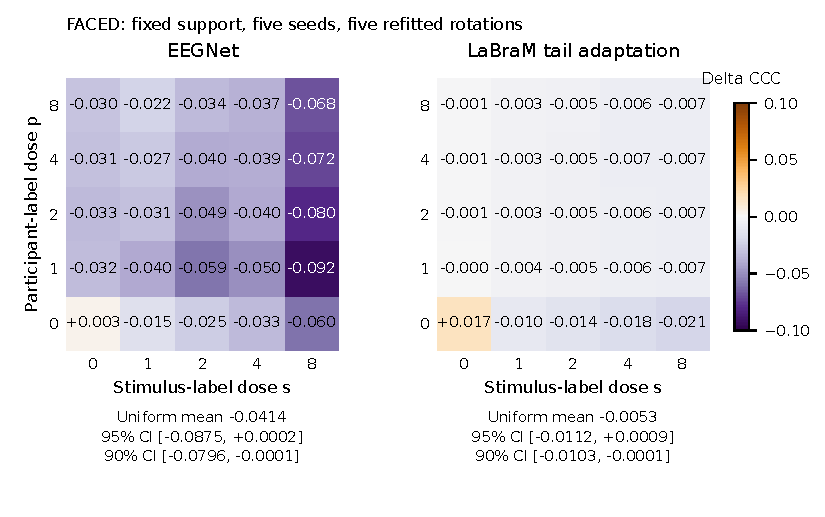
\includegraphics[width=\linewidth]{../generated/evidence_v14/faced_matched_heatmap.pdf}
\caption{The complete FACED matched-increment grids. Positive values favor EEG;
the shared scale and printed values retain dose heterogeneity. Displayed zeros
are rounded, not exact equality. Each cell
averages paired differences over executed seeds, rotations and targets on
identical test support. Intervals below each grid describe the uniform mean.
Pointwise and simultaneous cell bands are released separately; the heatmap
does not establish cellwise equivalence. Negative and failed positive controls
are reported in Table~\ref{tab:v14-controls}.}
\label{fig:faced-v14}
\end{figure}

% evidence: paper/generated/evidence_v14/resource_corners.csv
The heatmap exposes a boundary hidden by the mean. At zero participant
calibration, LaBraM's point increment changes from $+0.0170$ with no
same-stimulus labels to $-0.0212$ with eight such labels. At the corresponding
zero-stimulus corners, its increment is $+0.0170$ at participant dose zero and
$-0.0008$ at dose eight. All four corners for both architectures are released,
without choosing cells by sign. These are descriptive changes under different
contracts, not a tested causal effect of label acquisition or proof that a
particular cell has no EEG signal.

\subsection{Negative controls, failures and post-failure recovery}
% evidence: paper/generated/evidence_v14/all_results.csv; docs/confirmatory_positive_control_amendment_v14.md
Full-grid label permutations give mean increments $-0.0400$ (EEGNet) and
$-0.0058$ (LaBraM). Neither triggers the prespecified spurious-positive
warning; the similarity to observed estimates is descriptive, not a formal
observed-versus-permuted test. Two completed EEGNet sinusoidal positive
controls failed: raw-target encoding gave $-0.1476$, and residual-aligned
encoding gave $-0.0562$, below the required $+0.10$ gate. Thus target alignment
alone did not explain the failure. Both failures and their intervals remain
in Table~\ref{tab:v14-controls}.

% evidence: paper/generated/evidence_v14/all_results.csv; docs/confirmatory_positive_control_amendment_v14.md
After observing those failures, signed-power controls separated positive and
negative residual magnitudes across channels to avoid crop-dependent carrier
phase ambiguity. A frozen, cost-controlled subset recovered $+0.6512$ with
EEGNet and $+0.6303$ with LaBraM. It covers five selected splits, three stimulus
doses and all participant doses and training seeds, not the full crossed test
support. The earlier 52-fit incomplete full-grid attempt is retained and
excluded from inference. These results show sensitivity to a redesigned,
strong injected signal; they neither establish optimal use of real EEG nor
retroactively repair the failed locked controls. FACED is an unused cohort
with a prospectively locked observed-data design, but the complete pipeline
does not meet a fully preregistered confirmation claim.

\section{What the Evaluation Changes in Practice}
\label{sec:practical-cases}
% evidence: paper/generated/evidence_v14/system_attribution_cases.csv
\begin{table}[t]\centering\small
\caption{Existing maximum-dose LaBraM R1 cases: point CCC contrasts. Changing the comparator changes the attribution. None of the total or matched endpoint ranges establishes a positive gain; full conditional ranges and other settings are retained in the development appendix.}
\label{tab:v14-cases}
\begin{tabularx}{\linewidth}{@{}lXXX@{}}\toprule
Task & System $EC-P$ & Calibration $PC-P$ & Matched EEG $EC-PC$\\\midrule
EmoEEG-MC & $+0.0961$ & $+0.1420$ & $-0.0459$ \\
Urban & $+0.0587$ & $+0.0774$ & $-0.0186$ \\
\bottomrule\end{tabularx}
\end{table}

% evidence: paper/generated/evidence_argument_v10/decomposition_maximum_dose.csv
\paragraph{Case 1: attributing an apparent system gain.}
At the predeclared maximum resource dose, the frozen LaBraM R1 system improves
on the uncalibrated prior by $+0.0961$ CCC in EmoEEG-MC and $+0.0587$ in
Urban. Supplying exactly the same calibration labels to the EEG-free
comparator yields $+0.1420$ and $+0.0774$, leaving matched EEG differences
$-0.0459$ and $-0.0186$. The original positive point estimate describes the
system package; it does not identify added EEG value. Even the total-gain
intervals include zero, so this is not a reversal of an established
significant benefit. Appendix~\ref{app:development-v13} reports all settings
and the descriptive endpoint ranges. The practical correction is to change
the comparator and attribution, not to claim that a deployed sensor is
unnecessary.

% evidence: paper/generated/evidence_v14/resource_corners.csv; paper/generated/evidence_v14/all_results.csv
\paragraph{Case 2: distinguishing calibration regimes.}
A single zero-resource comparison cannot answer what EEG adds after repeated
stimulus labels become available. FACED's LaBraM surface ranges from positive
to negative point increments across those shared budgets, while its complete
uniform mean meets the fixed equivalence margins. Reporting the grid makes
the budget assumption visible and prevents promoting the mean to an
equivalence certificate for a selected deployment cell. This is the empirical
consequence of adding a stimulus axis to a participant-only baseline.

% evidence: paper/generated/submission_closure_v11/external_claim_repair.json; paper/generated/final_closure_v9/external_audit/public_summary.json
\paragraph{Case 3: narrowing an external execution claim.}
For the same pinned EEGain split function and eligible trial universe, the
checker blocks all five requests that jointly require held-out test
participants and training--validation trial isolation. The same five traces
allow the narrower held-out-test-participant claim. Generated marker windows
carry lineage only; no external emotion classifier was retrained. This
source-linked case changes a checkable claim about executed partitions, not
the validity of EEGain's published model scores. Separate synthetic faults
test resource parity and missing provenance; they are not attributed to
external authors. The reusable interface accepts trial identities, executed
resource records and explicit requirements, and returns \texttt{allow},
\texttt{block} or \texttt{unverifiable} with failed checks.


\section{Discussion, Limitations and Artifacts}
\paragraph{What is new, and what is not.}
Resource parity and identity-only baselines are established ideas. The proposed
object combines participant and stimulus label doses, fixed test support,
controlled population size and paired predictor outputs. Its value is the
additional conclusion it permits: whether a claimed component increment
persists under the stated calibration regime. It does not estimate a causal
neural mechanism, optimize an adaptation policy, or require every resource in
every benchmark to be identical. The matching contract must follow the
component named in the scientific claim.

% evidence: paper/generated/literature_resource_audit_v14/summary.json; paper/generated/literature_resource_audit_v14/ADJUDICATION_REPORT.md
\paragraph{Field relevance and the audit's limits.}
Two independently locked model-assisted coding passes found no eligible
learned no-EEG comparator in 24/24 publicly accessible EEG-affect papers.
This supports an exploratory observation about missing comparisons in that
cohort, not a claim that those papers used mismatched comparisons or reached
invalid conclusions. Access conditioning, search wording and correlated model
errors limit generalization; protocol unitization differs in four papers.
The source codes, disagreement records and post-lock adjudication are released
(Appendix~\ref{app:v14}). These automated passes do not satisfy a two-human
coding claim.

\paragraph{Limits of the scientific inference.}
Equal access does not ensure that the selected EEG architecture exploits the
resources optimally. Failed locked controls and post-failure signal redesign
remain material limitations even though later injected-signal recovery is
large. FACED intervals include the executed seed and rotation choices, not all
possible tuning or pretraining uncertainty. Older development intervals
condition on fitted models. Pre-outcome margins define a benchmark resolution,
not a clinically justified threshold; grid averaging can hide a useful cell,
target or participant subgroup. Repeated-stimulus budgets, label quality and
acquisition conditions differ between deployments. We establish neither an
economic advantage of avoiding EEG acquisition nor broad performance outside
the evaluated affect tasks. Cross-domain evidence motivates the transferable
contract, rather than validating mismatch prevalence in other fields.

% evidence: paper/generated/evidence_v14/archive_manifest.json; docs/v14_reproduction.md
\paragraph{Reproduction and responsible release.}
The v14 aggregate archive includes every completed neural analysis, all control
failures, resource-cell statistics, protocol amendments, hashes and deterministic
table-building code. The reviewer quickstart checks artifact integrity and
rebuilds tables without downloads, training or resampling. Raw-data reproduction
is separately documented for users with source access. The separately
instructed model operator's clean run remains author-assisted software
acceptance, not outside-person or full EEG-experiment reproduction. The
\href{https://anonymous.4open.science/\#!/r/OpenAffect-EEG-1815/}{anonymous code entry}
must resolve to this same v14 release at submission; an earlier file-access
check does not certify a later snapshot. We retain the current reference
template until the next venue's official format is published.

Recordings, individual features, trial predictions, stimulus media and fitted
weights remain with their original providers. Consent and source licenses
apply; Urban's inconsistent license wording is documented without mirroring
recordings. Identity probes measure exposure risks and must not be used for
re-identification. Self-report prediction is not access to a clinical state or
private emotion. Model assistance in literature coding and development is
explicitly disclosed; numerical predictions and contract checks are produced
by the documented estimators and deterministic code.

OpenAffect-EEG makes a system gain and an EEG increment different reportable
objects. Its strongest supported conclusion is specific: the comparator's
label resources change what the evaluated score contrast warrants, and
adapted LaBraM's average FACED increment meets the declared equivalence bounds
under a pipeline with disclosed control limitations. Uncertain and adverse
results remain visible instead of being converted into a universal verdict
about EEG.

% evidence: paper/neurips2026/main.tex
\label{main-content-end}
\bibliographystyle{plainnat}
\bibliography{../references}
\appendix
\setcounter{figure}{0}
\renewcommand{\thefigure}{S\arabic{figure}}
\renewcommand{\theHfigure}{appendix.\arabic{figure}}
\section{V14 Evidence, Frozen Analysis and Reproduction Boundaries}
\label{app:v14}
This appendix is the current v14 evidence layer. The following development
appendices preserve earlier analyses on their original supports. Their use of
``primary'' refers to their own frozen development plan, not to the prospective
FACED design. All v14 tables here are rebuilt from archived aggregate files;
the manuscript integration reruns no training, bootstrap or simulation.

\subsection{Pinned FACED acquisition and assignment}
% evidence: docs/confirmatory_faced_v14_protocol.md; docs/confirmatory_faced_structural_amendment_v14.md; docs/faced_ingestion_summary_v14.json; docs/faced_assignment_summary_v14.json
The source is FACED on NEMAR, nm000112 v1.1.3, under CC BY 4.0
\citep{chen2023faced,nemar2026faced}. The protocol was locked on 14 September
2026 before EEG samples or participant rating values were read. The cohort
contains 123 complete participants and 28 videos; all 3,444 trials pass the
complete-support rule without post-outcome exclusions. Eligibility requires
readable BDF, exactly one valid presentation of every video, at least 30 seconds
ending at video offset, finite ratings and finite selected EEG samples. No
rating is imputed and no outcome-dependent artefact rejection is performed.

% evidence: docs/confirmatory_faced_structural_amendment_v14.md; docs/faced_remote_preflight_summary_v14.json; docs/faced_signal_qc_summary_v14.json
Header-only preflight found 61 legacy and 62 modern channel schemas and
sampling rates of 1000 Hz (68 files) or 250 Hz (55 files). The pre-outcome
amendment renames legacy temporal channels and uses their common 30-channel
scalp intersection, excluding A1/A2 or horizontal EOG channels. Video end is
mapped to its nearest sample, then exactly 30 seconds are taken backwards.
After conversion to microvolts, common-average reference and a fourth-order
zero-phase 0.5--45 Hz Butterworth bandpass use two-second reflections of the
within-video window. Polyphase resampling yields 30 by 3,000 samples.
No post-video rating-period signal enters the padding. Ratings use
$(y-3.5)/3.5$. The Ridge view is per-channel log10 Welch power in five fixed
bands with a two-second window; it is a completed sanity baseline, not a new
neural model or a separately claimed confirmation result.

% evidence: paper/generated/evidence_v14/ridge_descriptive.csv
All 2,500 already executed Ridge cell records are retained as scalar metric
rows with source-record hashes. Their descriptive uniform mean is
$\FacedRidgeMean$ CCC (valence $-0.0052$, arousal $+0.0012$). These are means
of the existing cell scores; no new prediction or bootstrap was run. No joint
Ridge interval was archived, so we do not assign a significance or equivalence
decision to these point summaries.

% evidence: configs/confirmatory_faced_v14_experiment.yaml; docs/faced_assignment_summary_v14.json
Five participant folds and four stimulus folds give 20 test cross-products per
rotation. The five rotation seeds are 20260914, 20260931, 20260948, 20260965
and 20260982; the global split index runs from zero to 99. Population fitting
excludes test participants and initially excludes test stimuli; nonzero
stimulus doses add declared ratings from other participants by replacing donor
rows. Participant calibration remains outside population fitting. Each
rotation covers every eligible trial once, but rotations and seeds are not
additional independent participants. The recorded 17,220 rows per full-grid
cell count repeated trial occurrences across rotations; there are still only
3,444 distinct eligible trials and 123 independent participant identities.

\subsection{Neural training and uncertainty}
% evidence: scripts/run_eegnet_v14.py; scripts/run_labram_peft_v14.py; scripts/run_labram_finetune_v13.py; configs/confirmatory_faced_v14_experiment.yaml
EEGNet uses learning rates $10^{-3}$ and $10^{-4}$, dropout 0.25, AdamW weight
decay $10^{-4}$, batch size 128, at most 100 epochs and patience 15.
LaBraM adapts the final four transformer blocks, final normalization and a
linear regression head, with backbone/head learning rates $10^{-5}/10^{-3}$,
AdamW weight decay 0.01, batch size eight, at most 40 epochs and patience eight.
Training uses random ten-second crops; evaluation is deterministic. Validation
MAE selects duration, followed by full refitting on permitted training plus
validation trials. Training seeds are 2026091401 through 2026091405.
Participant-dose changes use post-fit calibration and do not cause redundant
EEG retraining. Checkpoints, pretraining exposure and arbitrary hyperparameter
search policies remain outside the observable claim contract.

% evidence: src/openaffect_eeg/training_uncertainty.py; paper/generated/evidence_v14/all_results.csv; docs/confirmatory_faced_v14_protocol.md
The analysis computes a CCC per target on each scoring split, pairs predictors
before averaging, and shares participant--stimulus multiplicities across
compared predictors and resource cells. Executed seeds and fully refitted
rotations are resampled within the frozen numerical procedure. Percentile 95\%
estimation intervals and 90\% TOST-compatible decision intervals use 2,000
requested draws; all full-grid stages have 2,000 valid draws and each
signed-power subset has 1,999. Cell CSVs additionally report MAE differences,
pointwise intervals and a max-absolute-deviation simultaneous band. This
bootstrap's coverage is not independently established by the older Gaussian
five-block simulations: those validate the older fixed-fit development
statistic only. Five seeds and five rotations also do not cover every possible
model, tuning strategy or acquisition domain.

% evidence: docs/confirmatory_faced_v14_protocol.md; paper/generated/evidence_v14/all_results.csv
The primary equivalence margin $\pm0.05$ and strict sensitivity margin
$\pm0.025$ were fixed before FACED label access. They operationalize two
absolute CCC resolutions, not a patient-, user- or task-validated minimum
important effect. We report the continuous estimate and both decision
intervals so readers can apply another justified bound. Equivalence is limited
to the average of the declared cells and targets. Older development datasets
have no prospective equivalence claim, and no FACED per-target or subgroup
equivalence is inferred from the pooled mean.

% evidence: paper/generated/evidence_v14/all_results.csv
\begin{table}[htbp]\centering\small
\caption{All completed FACED neural controls, including failures. Signed-power rows use an exploratory subset with 85 participants, 23 observed stimulus identities, 15 resource cells and five sampled split indices; they do not replace either failed full-grid control.}
\label{tab:v14-controls}
\begin{tabularx}{\linewidth}{@{}l l r X l@{}}\toprule
Model & Control & $\Delta$CCC & 95\% interval & Gate\\\midrule
EEGNet & label permutation & $-0.0400$ & $[-0.0856, +0.0002]$ & pass \\
LaBraM tail & label permutation & $-0.0058$ & $[-0.0077, -0.0041]$ & pass \\
EEGNet & raw-target sinusoid & $-0.1476$ & $[-0.2398, +0.0573]$ & warning \\
EEGNet & residual sinusoid & $-0.0562$ & $[-0.1193, +0.0267]$ & warning \\
EEGNet & signed-power subset & $+0.6512$ & $[+0.5968, +0.7854]$ & pass \\
LaBraM tail & signed-power subset & $+0.6303$ & $[+0.5770, +0.7595]$ & pass \\
\bottomrule\end{tabularx}
\end{table}


\subsection{Complete control chronology and source integrity}
% evidence: docs/confirmatory_positive_control_amendment_v14.md; paper/generated/evidence_v14/all_results.csv
The original raw-outcome sinusoid failed the EEGNet $+0.10$ recovery gate.
Because the model learns an outcome-minus-prior residual and adds it to the
prior, raw-target encoding could double-count that prior. The dated
17 September amendment encoded the residual, but the second completed control
also failed. A deterministic oracle residual attained $+0.6176$, showing the
gate is attainable under the scoring code, not proving neural learnability.
A subsequent single-cell signed-power pilot separated residual signs across
channels, reducing carrier phase ambiguity under random crops. This is a
post-failure mechanism hypothesis and diagnostic, not a preregistered test.

% evidence: docs/confirmatory_positive_control_amendment_v14.md; paper/generated/evidence_v14/all_results.csv
The signed-power full-grid attempt was stopped after 52 of 5,000 EEGNet
candidate fits because of measured cost; its partial record is excluded from
inference. Before the subset restart, split indices $0,20,40,60,80$, stimulus
doses $0,2,8$, all five participant doses and all five training seeds were
fixed. This yields 150 EEGNet candidates (75 selected) and 75 LaBraM fits. Its
realized support includes 85 participants and 23 videos. Both models recover
the redesigned signal, with the intervals in Table~\ref{tab:v14-controls};
neither replaces a failed full-grid control. The LaBraM full-grid permutation
has 2,500 fits and no spurious-positive warning. Completed controls, failed
controls, the stopped attempt and their different supports are disclosed
without changing observed predictions or original margins.

% evidence: paper/generated/evidence_v14/archive_manifest.json; paper/generated/evidence_v14/build_report.json
Ten completed neural analysis sets are released as immutable summary JSONs and
cell CSVs with source SHA-256 records. The paper builder checks every source
hash, complete cell key set, primary mean and equivalence decision before
formatting tables. Original machine fields labelled \texttt{confirmatory}
record the invocation scope; the paper's interpretation explicitly withholds
fully preregistered confirmation because the locked controls failed. A
resource-corner table retains every corner for both FACED architectures;
neither signs nor significance select the displayed cases. Ridge completion,
ingestion, structural-QC and assignment summaries are also released. Trial-level
predictions, participant identifiers, tensors and weights remain excluded.

\subsection{Model-assisted literature coding and independent execution}
% evidence: paper/generated/literature_resource_audit_v14/summary.json; paper/generated/literature_resource_audit_v14/ADJUDICATION_REPORT.md; docs/model_assisted_field_audit_v14.md
The literature sampling frame and coding manual were frozen before coding.
The original main/reserve cohort suffered access attrition; a dated amendment
continued the same hash order to form a 24-paper public-full-text sensitivity
cohort, four papers per year in 2021--2026. Two separately instructed model
operators locked their codes before comparison. Both found no eligible learned
no-EEG comparator in 24/24 papers. Raw agreement is 100\% for comparator
presence and parity, but Cohen's kappa is undefined for a constant category.
Claim type agreed in 23/24 papers; confidence agreed in 20/24. The operators
created 60 versus 57 protocol units; post-lock adjudication resolved omissions
and material splits for three papers, while one target-granularity choice
remains unresolved. No protocol-level kappa is inferred from unaligned units.
The coders share a model family and may share errors. This does not meet the
original two-human condition or estimate representative mismatch prevalence;
absence of a comparator is not evidence of an invalid comparison.

The separately instructed artifact operator used a clean Python environment.
The initial public quickstart exposed a stale release manifest; the controlled
builder and synchronized manifest repaired that failure. The final checks
verify executable software and aggregate evidence reconstruction, not full
raw-to-paper EEG retraining. The acceptance type remains
\texttt{author\_assisted}, with no independent-human claim. Model assistance
also supported coding, software maintenance and manuscript drafting; authors
are responsible for source checks and all scientific interpretations.

\subsection{Reproduction modes and computational boundary}
The reviewer quickstart validates the release, executes a synthetic contract
example, rebuilds earlier source-linked cases and rebuilds all v14 result
tables from the public aggregate archive. The following v14 command performs
only deterministic verification and formatting:
\begin{verbatim}
python scripts/build_v14_paper_assets.py --verify \
  --output /tmp/openaffect-v14-table-check
\end{verbatim}
Full scientific reproduction is a separate, explicit data-owner workflow:
obtain pinned source files, run the released signal/QC and assignment CLIs,
execute EEGNet or LaBraM with the frozen configurations, and run the joint
analysis on locally retained predictions. The command map, including all
failed controls and the fixed diagnostic subset, is in
\texttt{docs/v14\_reproduction.md}. The manuscript integration itself repeats
none of those experiments. Exact wall-clock and energy totals were not logged
consistently across all earlier runs, so no complete training-cost claim is
made. A remaining scientific limitation is that strong synthetic recovery
cannot establish sensitivity to all realistic EEG effects.

\section{Preserved Development Evidence and Diagnostics}
\label{app:development-v13}
These are the pre-v14 development analyses on their original supports. Fixed-fit
intervals and their simulation validation do not validate the FACED joint bootstrap.

\subsection{Evaluation coverage}
% evidence: paper/generated/final_closure_v9/verification/verification.json; configs/final_robustness_v9.json
We evaluate EmoEEG-MC (30 eligible participants, 42 stimuli; valence and
arousal) and Urban Appraisal (62 participants, 56 street images; genuine
valence trials only) \citep{openneuro_ds005540,openneuro_ds006850}.
Deterministic identity blocks test every eligible participant and stimulus once,
yielding 252 and 695 fixed test trials. The design tests five diagonal blocks,
not every possible participant--stimulus pair. Urban is an external appraisal
task, not an identical replication of emotion induction, and neither dataset is
an untouched confirmatory cohort.

Each task includes band-power Ridge, frozen LaBraM, and standard Braindecode
EEGNet \citep{jiang2024labram,lawhern2018eegnet}. Two bounded settings per model,
five identity blocks, and all 25 dose cells yield 1,500 model-cell results; these
cells are not independent observations. Ridge settings vary the candidate
regularization grid, while EEGNet settings vary learning rate. Validation
selects hyperparameters and training duration. Population refitting uses
training and validation trials but never test or calibration trials. We record
200 nonconstant EEGNet selection/refit histories as execution evidence, not as
proof of optimization. The Appendix reports full preprocessing, coverage,
budgets, and historical model panels.

% evidence: paper/generated/reviewer_revision_v12/learning_diagnostics.csv
The archived records show that, among 50 direct and 50 residual EEGNet fits per
task, 12/10 Emo and 8/7 Urban fits select epoch one; median selected epochs are
18/17.5 and 11/7.5. Training objectives decrease in the median for all four
groups. This rules out every network remaining at its initial fit, but does not
establish optimal tuning or a positive held-out EEG signal.

\subsection{A favourable total gain need not be an EEG gain}
\begin{table}[t]
\centering\small
\caption{Changing the comparison at the predeclared maximum dose $(p,s)=(8,8)$. Total system gain $EC-P$ includes the EEG-free calibration gain $PC-P$. The last column is the paired percentile interval for $EC-PC$, not a difference of interval endpoints. These descriptive endpoints do not replace the primary uniform-grid mean.}
\label{tab:resource-decomposition}
\begin{tabular}{@{}llrrrl@{}}
\toprule
Task & Setting & $EC-P$ & $PC-P$ & $EC-PC$ & Paired interval \\
\midrule
EmoEEG-MC & Band-power R1 & +0.1312 & +0.1420 & -0.0108 & [-0.0429, +0.0219] \\
EmoEEG-MC & Band-power R2 & +0.1318 & +0.1420 & -0.0102 & [-0.0403, +0.0206] \\
EmoEEG-MC & LaBraM R1 & +0.0961 & +0.1420 & -0.0459 & [-0.1098, +0.0139] \\
EmoEEG-MC & LaBraM R2 & +0.1325 & +0.1420 & -0.0095 & [-0.0419, +0.0243] \\
EmoEEG-MC & EEGNet L1 & +0.1400 & +0.1420 & -0.0020 & [-0.0065, +0.0027] \\
EmoEEG-MC & EEGNet L2 & +0.1420 & +0.1420 & 0.0000 & [-0.0040, +0.0043] \\
Urban & Band-power R1 & +0.0639 & +0.0774 & -0.0135 & [-0.0561, +0.0362] \\
Urban & Band-power R2 & +0.0643 & +0.0774 & -0.0131 & [-0.0398, +0.0199] \\
Urban & LaBraM R1 & +0.0587 & +0.0774 & -0.0186 & [-0.0563, +0.0126] \\
Urban & LaBraM R2 & +0.0689 & +0.0774 & -0.0085 & [-0.0373, +0.0172] \\
Urban & EEGNet L1 & +0.0885 & +0.0774 & +0.0111 & [-0.0147, +0.0360] \\
Urban & EEGNet L2 & +0.0851 & +0.0774 & +0.0078 & [-0.0064, +0.0252] \\
\bottomrule
\end{tabular}
\end{table}

% evidence: paper/generated/evidence_argument_v10/decomposition_maximum_dose.csv
Table~\ref{tab:resource-decomposition} applies the same predeclared maximum dose
to every setting. For EmoEEG-MC LaBraM R1, $EC$ improves on the uncalibrated
prior $P$ by $+0.0961$. Yet the same calibration labels improve the EEG-free
predictor by $+0.1420$, leaving a matched EEG difference of $-0.0459$
$[-0.1098,+0.0139]$. In Urban, the corresponding quantities are $+0.0587$,
$+0.0774$, and $-0.0186$ $[-0.0563,+0.0126]$. The system-level point gains are
positive; the EEG-specific contrasts are not established as positive. This is
the judgement that resource matching changes.

\begin{table}[t]
\centering\small
\caption{Primary uniform-grid mean matched EEG increment in CCC, with two-sided 95\% five-block $t$ intervals (df=4). Each task averages five fixed identity blocks and all 25 dose cells. Settings are sensitivity checks, not independent replications.}
\label{tab:primary-v13}
\begin{tabular}{@{}lll@{}}
\toprule
Setting & EmoEEG-MC: mean [interval] & Urban: mean [interval] \\
\midrule
Band-power R1 & -0.0069 [-0.0464, +0.0327] & -0.0060 [-0.0631, +0.0511] \\
Band-power R2 & -0.0091 [-0.0409, +0.0226] & -0.0069 [-0.0444, +0.0307] \\
LaBraM R1 & -0.0320 [-0.0883, +0.0242] & -0.0173 [-0.0607, +0.0261] \\
LaBraM R2 & -0.0137 [-0.0492, +0.0219] & -0.0035 [-0.0312, +0.0242] \\
EEGNet L1 & -0.0001 [-0.0065, +0.0064] & +0.0073 [-0.0117, +0.0264] \\
EEGNet L2 & +0.0003 [-0.0046, +0.0052] & +0.0086 [-0.0094, +0.0265] \\
\bottomrule
\end{tabular}
\end{table}

% evidence: paper/generated/final_revision_v13/block_t/table_added_value_summary.csv
The primary full-grid summaries in Table~\ref{tab:primary-v13} tell the same
bounded story: all 12 task--setting block-$t$ intervals include zero. The
conclusion is unchanged under released percentile, basic, and earlier t-normal
sensitivities. No equivalence margin was prespecified, so this does not establish
equivalence, universal reversal, absence of EEG information, or a ceiling on
future EEG methods. The secondary MAE contrast for LaBraM R1 indicates increased
error in both tasks under the primary construction; other configurations are
uncertain or interval-sensitive. Appendix~\ref{app:latest-evidence} reports all
CCC and MAE settings rather than selected rows.

% evidence: paper/generated/final_revision_v13/sensitivity/sensitivity_summary.json
Post-primary checks preserve that interpretation. An alternative identity
partition and complete refit shifts any point estimate by at most 0.0135 (Emo)
or 0.0154 (Urban), with all 12 intervals covering zero. Across three EEGNet
initialization schedules at the four resource corners, all 12 task--setting--run
intervals cover zero and the largest point span is 0.0097. Last-block LaBraM
residual fine-tuning gives $-0.0110$ [$-0.1041,+0.0820$] and $-0.0404$
[$-0.1159,+0.0351$]. These are bounded sensitivities run after the primary
analysis, not independent cohorts or an unconditional retraining interval.

% evidence: paper/generated/reviewer_revision_v12/figure_manifest.json
\begin{figure}[tp]\centering
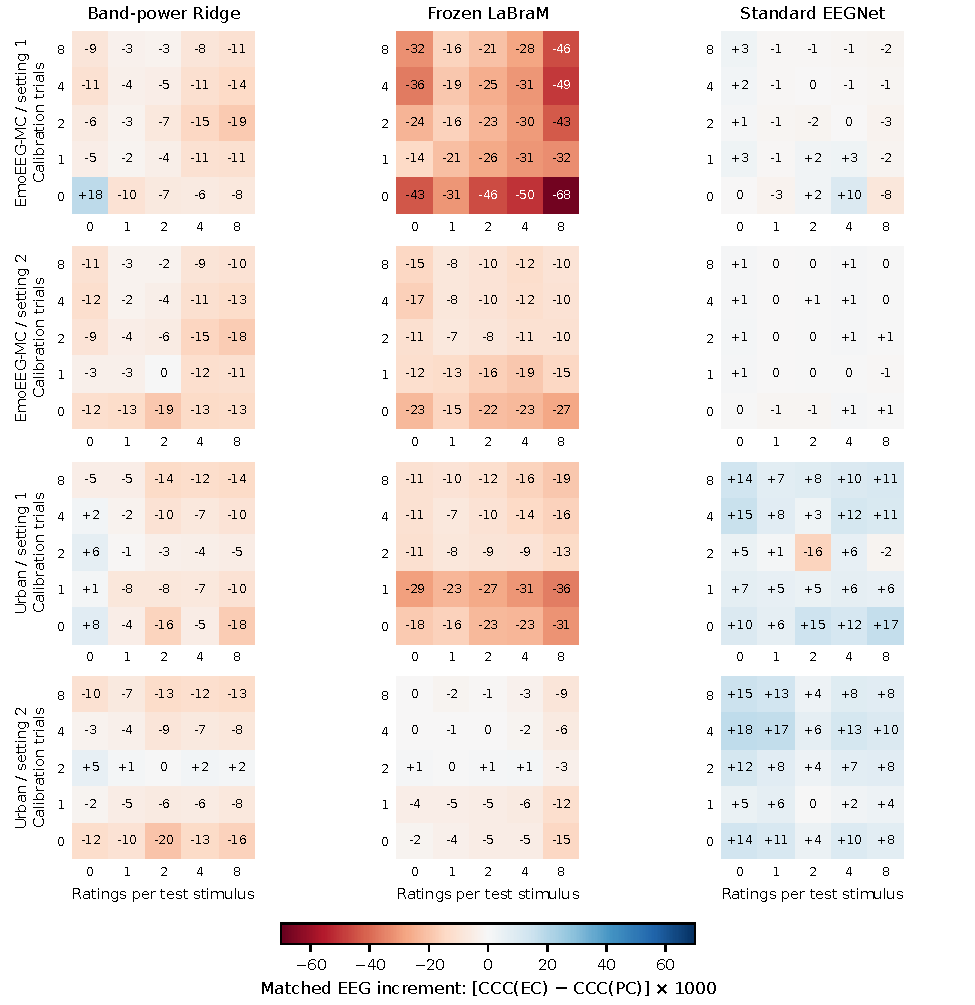
\includegraphics[width=\linewidth]{../generated/reviewer_revision_v12/matched_increment_heatmap.pdf}
\caption{All 12 matched-increment grids, with every dose retained. Entries and
color scale are $1000\Delta_{\rm EEG}$; rounded zero is not exact equality.
Rows distinguish tasks and settings (R1/L1, R2/L2); columns distinguish model
families. Positive values favor EEG. Each value averages five block-level
paired CCC contrasts. This is a descriptive display of already inspected
data, not an additional confirmatory test. Conditional pointwise stability
ranges and within-model dose-family bands accompany every cell in the released CSV.}
\label{fig:matched-grid}
\end{figure}

% evidence: paper/generated/reviewer_revision_v12/heterogeneity_summary.json
Figure~\ref{fig:matched-grid} exposes heterogeneity hidden by the uniform mean.
For example, Urban EEGNet L2 has positive point estimates in every cell, ranging
from $+0.0003$ to $+0.0177$; these do not establish positive increments at the
reported precision. None of the 300 cells has a positive pointwise CCC
range. Two Urban LaBraM R1 cells have negative pointwise ranges, but
neither survives its within-model dose-family band. These ranges are descriptive
because the cell estimands failed full calibration. We retain all 48
task--setting--corner comparisons $(0,0),(8,0),(0,8),(8,8)$ in a separate table;
no cell selection or averaging of interval endpoints is used.

% evidence: paper/generated/final_closure_v9/normal_t/table_added_value_summary.csv
Why is the matched comparator material? From zero dose, eight target-user
calibration trials increase EEG-free $PC$ CCC by $+0.2036$ in EmoEEG-MC and
$+0.1564$ in Urban. Eight other-participant ratings per test stimulus increase
it by $+0.4907$ and $+0.3408$, respectively; both interval constructions are
positive. The fact that labels help is unsurprising. Their magnitude relative
to the matched EEG contrasts shows why unequal label access can change the
attribution attached to a system score.

\subsection{Uncertainty and evaluator validity}
% evidence: paper/generated/final_closure_v9/percentile/added_value_statistics.json; paper/generated/final_closure_v9/normal_t/added_value_statistics.json
The crossed bootstrap applies identical participant and stimulus
multiplicities to every paired predictor, cell, and block. Of 2,000 draws, 1,985
are valid for EmoEEG-MC and 2,000 for Urban. The primary two-sided 95\% interval uses the
crossed-bootstrap standard error and a $t_{4}$ critical value because the final
estimand averages five predeclared identity blocks. Percentile, basic, and the
earlier within-block t-normal constructions are sensitivity checks. Every
construction conditions on fitted predictions and omits retraining uncertainty.
Pointwise ranges and separately released dose-family bands do not support
calibrated cell selection or all-model multiple comparisons.

% evidence: paper/generated/final_closure_v9/percentile/added_value_statistics.json
The relevant cluster sizes are those within each scoring block: Emo has six
participants and eight or nine stimuli per block; Urban has 12 or 13
participants and 11 or 12 stimuli. The whole-dataset participant count does
not by itself validate a mean of small-block CCCs. We therefore distinguish
the earlier single-block simulations below from the topology-matched
five-block check in Appendix~\ref{app:revision-diagnostics}.

% evidence: results/block_t_validation_v13/summary.csv; results/block_t_validation_v13/completion.json
The new topology-matched validation executes 300 replicates for each of four
Gaussian scenarios per task, with 2,000 bootstrap draws and no failed runs.
For the primary uniform mean, block-$t$ coverage is 0.993 for Emo and 1.000
for Urban under trial signal, and 0.980 and 0.983 under participant-constant
signal; the two non-signal checks cover at 1.000. The corresponding Wilson
Monte Carlo lower bounds are 0.957--0.987. The minimum cellwise coverage is
still 0.917, so this validation supports only the predeclared uniform mean.
The block-$t$ correction was introduced after the earlier interval diagnostics
failed, but its critical value follows the five-block aggregation and does not
use the observed EEG effect signs or magnitudes. Its evidence remains limited
to these four Gaussian families. We therefore make no calibrated cellwise,
equivalence, or unconditional retraining claim. Earlier single-block tests in
Appendix~\ref{app:evaluator-validation} cannot widen that scope.

\subsection{Scope checks and retained negative evidence}
Earlier EmoEEG-MC and MusicEEG surfaces, compact versus standard EEGNet,
CBraMod, LaBraM random controls, frozen EMOD, and calibration variants remain in
Appendix~\ref{app:exposure-surface}. They use distinct supports or protocols and
are not replications of the primary grid. The earlier MusicEEG LaBraM mean
increment is $\VThreeMusicMean$ [$\VThreeMusicLow,\VThreeMusicHigh$], an
uncertain auditory result that we retain rather than omit. Resource-conditioned
model selection likewise has no stable mean CCC benefit
(Appendix~\ref{app:selection-utility}).

Identity probes and subspace perturbations are representation diagnostics, not
causal evidence. The ds006866 analysis concerns condition exposure because
image identity is unavailable. DENS is missingness-limited; SEED-V is an
authorized aggregate supplement, not an openly redistributed benchmark. The
repaired EMOD single-seed check is neither a full original-task reproduction nor
evidence against EMOD, and mdJPT has no completed numerical audit here. These
records bound model and domain coverage; none is promoted to primary evidence.


\section{Development Resource-Matched Coverage Analysis}
\label{app:latest-evidence}
This section and the preserved development tables use the frozen
\texttt{final\_closure\_v9} evidence. The historical supplement preserves the original
experiments, figures, and their support. They are not additional independent
replications of this panel, and their historical use of ``primary'' denotes
their own frozen analysis plan rather than replacing the present main summary.

\subsection{Source and coverage details}
% evidence: configs/final_robustness_v9.json; paper/generated/final_closure_v9/verification/verification.json
EmoEEG-MC uses snapshot 1.0.7; Urban Appraisal uses snapshot 1.0.0
\citep{openneuro_ds005540,openneuro_ds006850}.
Emo has 1,260 eligible trials from 30 participants and 42 stimulus identities.
Urban uses 3,471 valence trials from 62 participants and 56 images; other
scales are not copied into valence/arousal labels. A source recording with
confirmed truncation was excluded before prediction inspection, as documented
in the frozen coverage manifest. Urban's dataset-description license says CC0,
while its README says CC BY 4.0. We document both declarations and do not
redistribute the source recording or image material.

% evidence: src/openaffect_eeg/final_robustness.py; configs/final_robustness_v9.json
SHA-256 ordering with design seed 20260908 assigns participant and stimulus
identities to five blocks. Block $b$ supplies test pairs; block $b+1$ modulo five
supplies validation pairs; population training initially uses identities from
the other blocks. Test pairs lie on diagonal blocks only. Coverage means every
eligible participant and stimulus is tested once, not every possible trial.
The same test support is retained throughout the dose grid. Stimulus-label
injection may use participants from the validation block; only the tested
participants are categorically excluded from population fitting at all doses.
This is not a claim of fully disjoint validation identities after injection.

\subsection{Bounded model settings and preprocessing}
% evidence: configs/final_robustness_v9.json; scripts/prepare_urban_tensors_v9.py; src/openaffect_eeg/final_robustness.py
Ridge R1 selects alpha from $\{0.1,1,10,100\}$ and R2 from
$\{1,10,100,1000\}$. Both band-power and frozen LaBraM use the two grids.
The historical Emo feature key \texttt{de} selects channel log-bandpower; it
does not make this panel a separate differential-entropy implementation.
Standard EEGNet is Braindecode 1.2.0 with F1=8, D=2, F2=16, dropout 0.25,
AdamW weight decay $10^{-4}$, batch size 128, at most 100 epochs and patience
15. L1 and L2 use learning rates $10^{-3}$ and $10^{-4}$. Validation MAE
selects training length; the selected length is refitted on train plus
validation. Both direct and residual branches are retained. Calibration changes
post-fit offsets only; it is not a sweep of few-shot fine-tuning algorithms.

% evidence: configs/final_robustness_v9.json; scripts/prepare_urban_tensors_v9.py
Emo uses the existing 100-Hz raw trial archive and ten-second EEGNet crops.
Urban uses 64 EEG channels in physical volts, excludes ECG and GSR, applies
common-average reference and polyphase resampling from 500 to 100 Hz, and
uses the three-second image interval before the rating response. At evaluation,
window predictions are averaged within a trial. Downstream learned
normalization is fitted without test or calibration trials. Frozen LaBraM
uses the project's recorded checkpoint and channel/unit adaptation; its upstream
training-data identity provenance is not certified here.

\subsection{Complete primary and secondary summaries}
% evidence: paper/generated/evidence_argument_v10/verification.json
All tables below are generated from the same hashed fitted predictions as the
main tables. The V13 primary interval recomputes the crossed bootstrap with a
five-block critical value; it performs no new fitting or model selection. The
score identity $EC-P=(PC-P)+(EC-PC)$ is checked
for all 300 task--setting--dose combinations after block aggregation, with
maximum numerical error below $10^{-12}$. This validates a numerical identity,
not a causal decomposition. Paired intervals are copied from paired contrast
outputs, never constructed by subtracting separate confidence bounds.
\begin{table}[htbp]\centering\small
\caption{EmoEEG-MC: uniform-grid EC-PC CCC. Paired pointwise intervals condition on fixed fitted predictions; t-normal is a heuristic sensitivity analysis.}
\begin{tabular}{@{}lrll@{}}\toprule
Setting & Mean & Percentile interval & t-normal interval \\
\midrule
Band-power R1 & -0.0069 & [-0.0333, +0.0221] & [-0.0435, +0.0298] \\
Band-power R2 & -0.0091 & [-0.0306, +0.0145] & [-0.0385, +0.0202] \\
LaBraM R1 & -0.0320 & [-0.0676, +0.0104] & [-0.0842, +0.0201] \\
LaBraM R2 & -0.0137 & [-0.0376, +0.0139] & [-0.0466, +0.0192] \\
EEGNet L1 & -0.0001 & [-0.0040, +0.0047] & [-0.0060, +0.0059] \\
EEGNet L2 & +0.0003 & [-0.0028, +0.0040] & [-0.0042, +0.0048] \\
\bottomrule\end{tabular}\end{table}
\begin{table}[htbp]\centering\small
\caption{EmoEEG-MC: uniform-grid EC-PC MAE. Paired pointwise intervals condition on fixed fitted predictions; t-normal is a heuristic sensitivity analysis.}
\begin{tabular}{@{}lrll@{}}\toprule
Setting & Mean & Percentile interval & t-normal interval \\
\midrule
Band-power R1 & +0.0047 & [-0.0004, +0.0099] & [-0.0019, +0.0113] \\
Band-power R2 & +0.0039 & [0.0000, +0.0078] & [-0.0013, +0.0090] \\
LaBraM R1 & +0.0151 & [+0.0061, +0.0242] & [+0.0034, +0.0269] \\
LaBraM R2 & +0.0065 & [+0.0016, +0.0112] & [+0.0001, +0.0129] \\
EEGNet L1 & +0.0002 & [-0.0008, +0.0013] & [-0.0012, +0.0016] \\
EEGNet L2 & +0.0002 & [-0.0004, +0.0009] & [-0.0007, +0.0011] \\
\bottomrule\end{tabular}\end{table}
\begin{table}[htbp]\centering\small
\caption{Urban: uniform-grid EC-PC CCC. Paired pointwise intervals condition on fixed fitted predictions; t-normal is a heuristic sensitivity analysis.}
\begin{tabular}{@{}lrll@{}}\toprule
Setting & Mean & Percentile interval & t-normal interval \\
\midrule
Band-power R1 & -0.0060 & [-0.0432, +0.0376] & [-0.0519, +0.0398] \\
Band-power R2 & -0.0069 & [-0.0312, +0.0216] & [-0.0370, +0.0233] \\
LaBraM R1 & -0.0173 & [-0.0482, +0.0112] & [-0.0522, +0.0175] \\
LaBraM R2 & -0.0035 & [-0.0238, +0.0150] & [-0.0257, +0.0187] \\
EEGNet L1 & +0.0073 & [-0.0056, +0.0217] & [-0.0080, +0.0226] \\
EEGNet L2 & +0.0086 & [-0.0043, +0.0215] & [-0.0059, +0.0230] \\
\bottomrule\end{tabular}\end{table}
\begin{table}[htbp]\centering\small
\caption{Urban: uniform-grid EC-PC MAE. Paired pointwise intervals condition on fixed fitted predictions; t-normal is a heuristic sensitivity analysis.}
\begin{tabular}{@{}lrll@{}}\toprule
Setting & Mean & Percentile interval & t-normal interval \\
\midrule
Band-power R1 & +0.0063 & [-0.0012, +0.0144] & [-0.0024, +0.0151] \\
Band-power R2 & +0.0037 & [-0.0009, +0.0082] & [-0.0015, +0.0089] \\
LaBraM R1 & +0.0091 & [+0.0036, +0.0148] & [+0.0027, +0.0156] \\
LaBraM R2 & +0.0038 & [+0.0003, +0.0073] & [-0.0002, +0.0078] \\
EEGNet L1 & +0.0027 & [-0.0009, +0.0068] & [-0.0016, +0.0071] \\
EEGNet L2 & +0.0012 & [-0.0013, +0.0041] & [-0.0019, +0.0043] \\
\bottomrule\end{tabular}\end{table}


\subsection{Resource effects and statistical limits}
% evidence: paper/generated/final_closure_v9/normal_t/table_added_value_summary.csv
For the EEG-free prior, participant-dose changes from $(0,0)$ to $(8,0)$ are
$+0.2036$ $[+0.0955,+0.3116]$ on Emo and $+0.1564$ $[+0.0492,+0.2637]$ on
Urban. Stimulus-dose changes to $(0,8)$ are $+0.4907$ $[+0.3581,+0.6233]$ and
$+0.3408$ $[+0.2161,+0.4655]$. Joint changes to $(8,8)$ are $+0.6327$
$[+0.4810,+0.7844]$ and $+0.4181$ $[+0.2928,+0.5435]$. These are heuristic
t-normal sensitivity intervals; the corresponding percentile intervals also
exclude zero. They are not the same contrasts as $PC-P$ at a fixed stimulus
dose in the main endpoint table.

The bootstrap reuses crossed participant and stimulus multiplicities across
all fitted predictors. Averages are computed within block and then across
blocks rather than pretending repeated grid predictions are new observations.
The finite-cluster coverage diagnostics and invalid-draw counts constrain
interpretation. The primary block-$t$ interval addresses the uniform-grid mean
only and remains a fixed-fit uncertainty summary, not a repeated-training
confidence statement or equivalence test. Neither isolated pointwise
ranges nor dose-family bands imply simultaneous coverage over every method,
task, and secondary endpoint inspected during benchmark development.

\subsection{Known-truth evaluator stress tests}
\label{app:evaluator-validation}
% evidence: paper/generated/submission_closure_v11/evaluation_method_validation.json
We tested the estimator on outcomes with known construction before interpreting
the EEG results. In the v6 oracle suite, 16 settings with 100 replicates each
produced the following operating characteristics. ``Detection'' denotes a
strictly positive interval and is not a universal power guarantee.

\begin{center}
\small\setlength{\tabcolsep}{4pt}
\begin{tabularx}{\linewidth}{>{\raggedright\arraybackslash}p{0.19\linewidth}>{\raggedright\arraybackslash}p{0.23\linewidth}>{\raggedright\arraybackslash}X}
\toprule
Generator & Recorded behavior & Interpretation boundary \\
\midrule
Labels only & mean difference exactly zero & algebraic negative control only \\
Independent noise & 0/16 cells detected & finite evidence, not a proof of zero false positives \\
Trial signal & detection 0.85--1.00; coverage 0.92--1.00 & detects the injected trial signal in these settings \\
Participant constant & minimum coverage 0.82 & exposes finite-cluster weakness; no biological or causal interpretation \\
\bottomrule
\end{tabularx}
\end{center}
% evidence: paper/generated/submission_closure_v11/evaluation_method_validation.json

The v7 finite-cluster study planned 9,600 fits; 9,584 were valid and 16 were
rejected by the declared support rule. In the target $32\times24$ cluster
setting, percentile, basic, and t-normal coverages were 0.933, 0.930, and
0.957. Their minima in the deliberately small $8\times6$ setting were 0.837,
0.820, and 0.940. The often wider t-normal interval is therefore retained as
a sensitivity analysis, not promoted as a generally calibrated solution.
% evidence: paper/generated/submission_closure_v11/evaluation_method_validation.json

\subsection{Rule basis and three-state decisions}
% source: configs/audit_rule_catalog.json
The checker implements observable evidence rules rather than inferring
scientific validity from a score. Every rule returns allow, block, or
unverifiable; the last state is preserved when required provenance is absent.

\begin{center}
\small\setlength{\tabcolsep}{4pt}
\begin{tabularx}{\linewidth}{>{\raggedright\arraybackslash}p{0.18\linewidth}>{\raggedright\arraybackslash}p{0.27\linewidth}>{\raggedright\arraybackslash}X}
\toprule
Rule family & Required evidence & Example boundary \\
\midrule
Trial lineage & trial UIDs in every partition & repeated derived windows block trial-isolation claims \\
Identity holdout & participant/stimulus UIDs & overlap blocks only the identity claim it violates \\
Preprocess/selection & fit and selection UIDs & missing provenance is unverifiable, not a pass \\
Matched resources & predictor-specific label access & unequal calibration blocks an EEG-added-value claim \\
Fixed support & test-set hashes by comparator & unequal test support blocks a paired comparison \\
\bottomrule
\end{tabularx}
\end{center}
These rules operationalize documented leakage and benchmark-reporting concerns
\citep{brookshire2024leakage,lei2025leakage,bendrich2022feature,reuel2024betterbench};
they do not certify data truth, upstream pretraining history, or causal validity.

\section{Source-Linked Execution Cases and Reuse}
\label{app:execution-cases}
% evidence: paper/generated/final_closure_v9/external_audit/public_summary.json
The executed EEGain commit is
\texttt{d6892f5586181f345969651a9baedabd828bb1c5}; its
\texttt{EEGDataloader.split\_train\_val} is in
\texttt{eegain/data/loader.py}. LibEER is pinned to
\texttt{dddff9776dbdae21195fe320dff0a5ba61628a18}; we execute
\texttt{get\_split\_index}, \texttt{index\_to\_data}, and the empty-validation
branch at lines 100--102 of \texttt{LibEER/EEGNet\_train.py}.
File hashes, selected source ranges, case origin, and outputs are recorded in
\texttt{external\_audit/public\_summary.json} and its paired case table.
Marker windows are generated from real trial identities, not independent EEG
measurements. No external classifier score is inferred from the branch tests.

The same EEGain execution record produces different answers to different
contracts: its held-out test participants remain excluded, while an additional
requirement that validation trials be disjoint from training can be violated.
Changing the claim to what was actually isolated is one valid repair. When a
strict validation-trial contract is required, partitioning complete trials
before generating windows is the appropriate construction instead. LibEER's
explicit train/validation/test path passes the exercised split checks; its
empty-validation fallback should not be treated as independent validation.
The machine-readable repair record
\texttt{submission\_closure\_v11/external\_claim\_repair.json} verifies this
strict-block/scoped-allow pair across all five exercised EEGain folds while
holding the pinned function, trial universe, and execution output fixed. The
repair changes the supportable claim; it does not alter or re-estimate a model
score.

\begin{small}\begin{verbatim}
python scripts/run_workflow_contract_toy.py toy_contract
python -m openaffect_eeg.workflow_audit \
  --trials toy_contract/trials.tsv \
  --execution toy_contract/unmatched_calibration_execution.json \
  --contract toy_contract/unmatched_calibration_contract.json \
  --output toy_contract/checked.json
\end{verbatim}\end{small}
The mismatch example exits with the documented blocked status; the matched
example passes observable checks. Omitting preprocessing evidence preserves
uncertainty. This is a developer-operated executable example, not independent
human acceptance. The checker validates consistency of supplied execution
records, not adversarially falsified provenance.

\paragraph{AI-assisted development.}
AI assistance was used for protocol and code drafting, debugging, literature
triage, analysis support, and manuscript development. The recorded EEG
predictions, bootstrap summaries, and contract decisions are generated by
the documented numerical models and deterministic checks, not by an LLM
acting as an emotion predictor or audit judge. Automated checks and agent-run
examples are not independent human review. Authors remain responsible for
source verification, scientific interpretation, and submission approval.


\section{Matched-Grid Display and Learning Diagnostics}
\label{app:revision-diagnostics}

\subsection{Complete cell evidence and deployment interpretation}
% evidence: paper/generated/reviewer_revision_v12/figure_manifest.json
The display in Figure~\ref{fig:matched-grid} is generated directly from
\texttt{table\_added\_value\_contrasts.csv}. It preserves all 300
task--setting--dose rows, with their paired pointwise CCC/MAE intervals and
within-model dose-family CCC bands. The four resource corners give 48
comparisons across all settings, including unfavorable and uncertain results.
The files \texttt{matched\_increment\_all\_cells.csv} and
\texttt{deployment\_corners.csv} retain unrounded values. A common symmetric
color scale is used, with entries multiplied by 1000 for legibility.
The visualization was added after examining the results and is descriptive.

The four corners answer different deployment questions: no target-user
calibration or repeated-stimulus ratings; calibration only; repeated-stimulus
ratings only; and both. Released normative information remains separately
declared. These scenarios do not make ratings costless or assert that stimuli
will recur in a real application. A weighted application score requires
weights selected for that application and paired prediction-level uncertainty.
Marginal interval endpoints cannot be averaged to obtain such an interval.

\subsection{Real-task optimization evidence}
% evidence: paper/generated/reviewer_revision_v12/learning_diagnostics.csv
\begin{table}[ht]\centering\small
\caption{Previously executed EEGNet training diagnostics, now summarized by
task and branch. Counts refer to settings, identity blocks, and stimulus doses,
not independent participants or studies. Objective reduction is the median
initial-minus-final recorded training objective; these values are not test
metrics and are not comparable performance measures across tasks.}
\begin{tabular}{llrrrr}\toprule
Task & Branch & Fits & Epoch-one & Median epoch & Objective reduction\\\midrule
Emo & Direct & 50 & 12 & 18 & 0.1104\\
Emo & Residual & 50 & 10 & 17.5 & 0.1162\\
Urban & Direct & 50 & 8 & 11 & 0.1922\\
Urban & Residual & 50 & 7 & 7.5 & 0.2080\\
\bottomrule\end{tabular}
\end{table}
These aggregates come from the same verification record as the primary
predictions, not from newly selected runs. The historical standard/compact
EEGNet and matched shrinkage-calibration comparisons remain supporting
evidence on their original supports. The repaired real SEED-V task provides
a separate compatibility check, not a positive control for the current
self-report regression task. None of these records spans full fine-tuning,
all calibration algorithms, or repeated-training uncertainty. The scope of
the matched increment remains the specified fitted predictor pair.

\subsection{Post-primary partition, initialization, and fine-tuning checks}
% evidence: paper/generated/final_revision_v13/sensitivity/sensitivity_summary.json; paper/generated/final_revision_v13/sensitivity/finetune_execution
\begin{table}[ht]\centering\small
\caption{Post-primary robustness checks. Block-$t$ intervals remain conditional on each fitted run. Alternative partitions and initialization schedules are sensitivity analyses, not independent cohorts.}
\begin{tabularx}{\linewidth}{p{0.09\linewidth}p{0.22\linewidth}p{0.18\linewidth}X}\toprule
Task & Check & Setting & Result\\\midrule
Emo & New blocks + refit & Six settings & max point shift 0.0135; 6/6 cover 0\\
Urban & New blocks + refit & Six settings & max point shift 0.0154; 6/6 cover 0\\
Emo & Three train seeds & EEGNet L1 & [-0.0094, -0.0015]; 3/3 cover 0\\
Emo & Three train seeds & EEGNet L2 & [-0.0018, +0.0003]; 3/3 cover 0\\
Urban & Three train seeds & EEGNet L1 & [+0.0097, +0.0134]; 3/3 cover 0\\
Urban & Three train seeds & EEGNet L2 & [+0.0013, +0.0109]; 3/3 cover 0\\
Emo & Last-block fine-tune & LaBraM residual & -0.0110 [-0.1041, +0.0820]\\
Urban & Last-block fine-tune & LaBraM residual & -0.0404 [-0.1159, +0.0351]\\
\bottomrule\end{tabularx}
\end{table}

The alternative partition repeats assignment, fitting, aggregation, and
verification with a new design seed; because the fitted data also change, it is
a partition/refit sensitivity rather than an isolated partition effect. The
three EEGNet schedules share the original assignments and four resource
corners, changing only declared training initialization offsets. The LaBraM
check uses the official checkpoint, freezes all but the final transformer block
and normalization, fits a residual head, selects epochs on validation data, and
then refits on training plus validation. Its 100-Hz analysis tensors are
linearly resampled to the official 200-Hz patch interface; the Urban voltage
conversion is checked from recorded metadata. All checks condition their
block-$t$ intervals on the resulting fitted predictions. They were specified
after the primary results, cover neither a new cohort nor the full $5\times5$
fine-tuning surface, and cannot certify invariance to arbitrary partitions,
optimizers, checkpoints, or adaptation methods.

\subsection{Five-block interval validation}
The production statistic first computes paired CCC differences within each
identity block, then averages blocks and dose cells. It does not pool all
trials before computing CCC. The new validation implementation preserves this
order and uses the same global participant and stimulus multinomial weights
across all blocks and cells. A draw invalid in any block is not repaired by
omitting that block. Tests compare its cell estimates, uniform means, interval
endpoints, and valid-draw counts with the production analyzer for both one-
and two-target tasks.

% evidence: configs/block_validation_v12.json; paper/generated/final_closure_v9/percentile/added_value_statistics.json
The frozen validation configuration uses the exact complete diagonal test
supports in the primary verification record: $6\times9,6\times9,6\times8,
6\times8,6\times8$ for Emo, and $13\times12,13\times11,12\times11,
12\times11,12\times11$ for Urban. It retains the full $5\times5$ dose grid,
two targets for Emo and one for Urban. Four previously defined Gaussian
scenarios exercise label-only cancellation, trial signal, participant-constant
signal, and independent noise. Each scenario uses 300 fresh simulation
replicates per task and 2,000 bootstrap draws. The primary block-$t$ interval
retains the crossed-bootstrap standard error and uses the five identity blocks
as the independent aggregation units (df=4). Percentile, basic, and the earlier
within-block t-normal intervals remain sensitivity checks. The correction was
introduced after the initial interval diagnostics failed, but its critical
value is fixed by the estimand topology and does not use the real EEG effect
signs or magnitudes.

The estimand is the scenario's analytic population matched CCC difference,
averaged uniformly over dose cells. Finite-block estimation bias is part of
the stress test. Synthetic block resources are independent: matching this
test topology does not reproduce all cross-block training-resource dependence,
the actual EEG distribution, or retraining uncertainty. Coverage proportions
require Monte Carlo uncertainty and do not establish validity outside the
tested constructions. Executed results are recorded in the accompanying
validation artifact.


% evidence: results/block_t_validation_v13/summary.csv; results/block_t_validation_v13/completion.json
\begin{table}[ht]\centering\small
\caption{Coverage of the primary uniform-grid mean under the observed five-block topology (300 replicates per row). Brackets give Wilson Monte Carlo intervals for the primary block-$t$ coverage.}
\begin{tabular}{llccc}\toprule
Task & Scenario & Block-$t$ [MC interval] & Percentile & Basic\\\midrule
Emo & Trial signal & 0.993 [0.976, 0.998] & 0.900 & 0.983\\
Emo & Participant constant & 0.980 [0.957, 0.991] & 0.903 & 0.910\\
Emo & Independent noise & 1.000 [0.987, 1.000] & 1.000 & 1.000\\
Emo & Labels only & 1.000 [0.987, 1.000] & 1.000 & 1.000\\
Urban & Trial signal & 1.000 [0.987, 1.000] & 0.927 & 0.977\\
Urban & Participant constant & 0.983 [0.962, 0.993] & 0.970 & 0.920\\
Urban & Independent noise & 1.000 [0.987, 1.000] & 1.000 & 1.000\\
Urban & Labels only & 1.000 [0.987, 1.000] & 1.000 & 1.000\\
\bottomrule\end{tabular}
\end{table}

All 2,400 simulation replicates completed without a failed run. The original
187,200 candidate rows and 62,400 derived block-$t$ rows include every cell and
uniform mean; they are not 249,600 independent simulations. Labels-only cancellation gives degenerate
zero differences; its coverage of one is an algebraic check, not calibration
of a nondegenerate interval. Independent noise produces no positive interval
in these runs, which does not establish false-positive control for every null.

% evidence: results/block_t_validation_v13/summary.csv; paper/generated/reviewer_revision_v12/five_block_all_coverage.csv
The earlier percentile failure is substantive. At Emo's zero-dose
participant-constant cell, its population-target bias is $-0.0756$ and coverage
is $0.193$ (Monte Carlo interval $[0.153,0.242]$); the earlier t-normal coverage
is $0.887$. The block-$t$ construction raises the minimum cell coverage to
$0.917$, which still does not validate cellwise inference. Its uniform-mean
coverage is $0.980$--$1.000$ across the eight task--scenario combinations, with
Wilson lower bounds of $0.957$--$0.987$. These tests support the primary
uniform-grid mean under the simulated topology, not every cell, the actual EEG
distribution, arbitrary signal families, or retraining uncertainty. Resource
identity and descriptive paired differences do not depend on a nominal
significance threshold; no equivalence claim is made.

\clearpage
% constants-source: paper/neurips2026/supplement.tex
\section*{Historical Supporting Analyses}
These analyses retain their original test supports and estimators. They are supporting records, not independent replications of the current primary grid. The current design and diagnostics precede this historical supplement.

\section{Data Sources and Trial Reconstruction}
\label{app:data}

\subsection{Version-pinned sources}

OpenAffect-EEG uses fixed OpenNeuro snapshots rather than a floating latest
version: MusicEEG ds002721 version 1.0.3, DENS ds003751 version 1.0.6,
EmoEEG-MC ds005540 version 1.0.7, and external validation ds006866 version
1.0.0
\citep{openneuro_ds002721,openneuro_ds003751,openneuro_ds005540,openneuro_ds006866}.
Snapshot manifests, byte counts or annex keys, and derived trial-table hashes
record the source state. Across the \claimvalue{C39} datasets we reconstruct
\claimvalue{C41} trials from \claimvalue{C40} dataset-qualified participants;
\claimvalue{C42} trials have complete harmonizable continuous targets. The core
tier contains \claimvalue{C35} participants, \claimvalue{C36} trials,
\claimvalue{C37} qualified stimulus identities, and \claimvalue{C38} supervised
trials.

\begin{table}[t]
  \caption{Source and redistribution boundaries. License entries describe the
  fixed source metadata; companion media and code retain separate terms.}
  \label{tab:licenses}
  \centering
  \small
  \setlength{\tabcolsep}{4pt}
  \begin{tabularx}{\linewidth}{@{}lXXX@{}}
    \toprule
    Dataset & OpenNeuro snapshot & Companion boundary & Benchmark release \\
    \midrule
    MusicEEG & CC0 & OSF metadata/audio: CC BY 4.0 & Metadata, splits, scores \\
    DENS & CC0 field; ODbL/DbCL conflict & Videos not mirrored & Conservative attribution \\
    EmoEEG-MC & CC0 & Stimuli/code/checkpoints separate & No EEG, DE, media, weights \\
    ds006866 & CC0 & OSF table: CC BY 4.0; source images separate & No EEG or images \\
    \bottomrule
  \end{tabularx}
  % evidence: fixed dataset_description.json files; paper/generated/table_benchmark_scope.csv
\end{table}

\begin{table}[t]
  \caption{Observed-data and probe-coverage disclosure. EEG feature counts are
  applied after a frozen trial assignment; missing signals never redefine a
  split. Probe coverage is the test fraction whose class was observed in fit.}
  \label{tab:coverage}
  \centering
  \small
  \setlength{\tabcolsep}{4pt}
  \begin{tabularx}{\linewidth}{@{}lrrXr@{}}
    \toprule
    Dataset & Labeled & EEG features & Main role & Stimulus probe \\
    \midrule
    MusicEEG & 1,240 & 1,240 & Transparent spectral audit & 0.8708 \\
    DENS & 365 & 162 & Transparent, missingness-limited & 0.9826 \\
    EmoEEG-MC & 1,260 & 1,260 & DE and foundation case study & 1.0000 \\
    ds006866 & 35,504 & 35,504 & Condition-level external audit & N/A \\
    \bottomrule
  \end{tabularx}
  % evidence: paper/generated/table_benchmark_scope.csv; paper/generated/table_identity_probes.csv
\end{table}

The DENS gap originates from unreadable public signal windows rather than an
explicit target filter, but the resulting complete-case set is not ignorable.
Only \claimvalue{C75} of \claimvalue{C76} label-eligible trials are available
(missing fraction \claimvalue{C74}); \claimvalue{C78} participants have no
available trial, and the available-versus-missing valence standardized mean
difference is \claimvalue{C77}. Missingness summaries and probe seen-class
fractions are published per dataset and seed. Subject probes in the LaBraM case study have complete test
coverage; permutation labels are shuffled only in the training partition while
the assignment, features, estimator, and test labels remain fixed.

\paragraph{MusicEEG.}
Participants listened to film-music excerpts and completed eight self-report
items \citep{daly2020musiceeg}. The benchmark retains 1,240 task trials. Public
events do not directly provide canonical audio filenames, so
\texttt{stimulus\_uid} is aligned from event codes to the public OSF Set 1 after
checking uniqueness, code range, and the availability of audio and normative
ratings for every candidate. Because the README, event description, and early
paper do not fully agree on the material set, this mapping is labeled
\texttt{audited\_inference}, not \texttt{source\_verified}. The OpenNeuro
snapshot declares CC0 and the companion OSF resource declares CC BY 4.0; audio
is not redistributed. % evidence: paper/generated/table_benchmark_scope.csv; cards/datasets/ds002721.md

\paragraph{DENS.}
DENS uses naturalistic videos and collects dimensional and categorical ratings
\citep{asif2023dens}. Events and behavior are joined by normalized stimulus
name, never row position. Several public \texttt{.fdt} lengths disagree with
their \texttt{.set} headers; unreadable full windows are recorded through an
availability mask rather than padded, wrapped, or treated as valid EEG. Public
events contain twenty local stimulus names, but the snapshot lacks the
documented stimulus and code directories, and the cited AFDI entry cannot be
reliably linked to those local identities. They are therefore valid grouping
keys but not claims of recovered source films. Conflicting CC0 and ODbL/DbCL
statements are handled under the more conservative attribution and share-alike
boundary. % evidence: paper/generated/table_benchmark_scope.csv; cards/datasets/ds003751.md

\paragraph{EmoEEG-MC.}
The dataset combines video viewing and text-guided imagery
\citep{xu2025emoeeg}. A published behavioral \texttt{video\_name} field repeats
one erroneous value for some participants and cannot be joined by row order.
The supervised subset is restricted to globally verifiable stimulus codes, and
context direction is cross-checked against source EDF trigger types. Other
reconstructed trials remain in provenance with unavailable targets. Public DE
arrays, reordered EEG, model features, and checkpoints are excluded from the
anonymous package. % evidence: cards/datasets/ds005540.md

\paragraph{External emotion regulation.}
ds006866 studies social and nonsocial images under neutral viewing, negative
viewing, and reappraisal conditions \citep{maka2026discrepancy}. It contributes
\claimvalue{C43} participants and \claimvalue{C44} image-presentation trials,
of which \claimvalue{C33} have complete valence and arousal. Public events
recover condition but not trial-level image identity, and EEGLAB annotations do
not restore it. Stimulus and joint holdout are consequently blocked by source
metadata. The OpenNeuro snapshot declares CC0; companion metadata declare CC BY
4.0, while source images can have separate terms. Neither images nor a
substitute media index are distributed. % evidence: cards/datasets/ds006866.md

\section{Target Harmonization}

MusicEEG pleasantness and energetic-arousal reports define valence and arousal;
the other datasets use their released valence and arousal fields. MusicEEG,
DENS, and ds006866 map an original one-to-nine scale by $(x-1)/8$; EmoEEG-MC
maps zero-to-seven by $x/7$. Original values, scale labels, and transformation
expressions remain in trial metadata or result provenance.
% constants-source: src/openaffect_eeg/baselines.py

The supervised target is the participant's trial-level report. Nominal stimulus
category, normative rating, and experimental condition can be inputs,
stratification variables, or audit labels, but do not replace the participant
target. Trials missing either continuous dimension remain in metadata and are
excluded only from metrics requiring both dimensions.

\section{Split Protocols}
\label{app:splits}

\paragraph{Single-factor protocols and the optimistic control.}
Complete trials are assigned before windowing. Random-trial, subject, and
stimulus holdout use 70/10/20 train/validation/test proportions within each
dataset, with at least one identity reserved for validation and test in small
groups. Random-trial splitting isolates only \texttt{trial\_uid} and records
subject and stimulus overlaps. Strict single-factor splits require an empty
train--test intersection for the held identity.
% constants-source: src/openaffect_eeg/splits.py; scripts/build_strict_splits.py

\paragraph{Joint holdout.}
Subjects and stimuli are independently assigned 60/20/20. A trial is retained
only when both identities receive the same partition; cross-partition edges are
marked \texttt{excluded}. This sacrifices coverage in sparse subject--stimulus
graphs to obtain a genuine double cold start. The ratio was fixed before model
evaluation because smaller validation identity sets did not provide adequate
validation coverage across seeds.
% constants-source: scripts/build_strict_splits.py

\paragraph{Support-matched identity-overlap control.}
For each joint-holdout seed, the control freezes the exact test trial IDs and
matches the joint split's train and validation row counts. It then samples those
training-side rows so that both test subjects and test stimuli occur in the fit
partition. Consequently, the control preserves test support and sample counts
while changing training-side identity overlap and the associated graph. It is
an estimand for the practical effect of available identity structure, not a
claim that all higher-order graph properties are identical.
Across seeds, test sets contain \claimvalue{C79}--\claimvalue{C80} trials from
\claimvalue{C81}--\claimvalue{C82} participants and exactly
\claimvalue{C83} held-out stimuli.
% constants-source: src/openaffect_eeg/reviewer_controls.py; scripts/build_support_matched_control.py

% constants-source: paper/figure_plan_zh.json
\placeholderfigure{figures/figureS_protocol_audit.pdf}{2.20in}{Protocol-level
audit retained as supporting evidence. \textbf{A:} five fixed split seeds and
their mean macro-CCC for semantic prior, direct EEG, and prior-plus-EEG residual;
random-trial splitting is an optimistic control. \textbf{B:} pretrained versus
fixed-random LaBraM comparisons and support-matched identity-overlap effects.
These estimates motivate the response-surface analysis but do not by themselves
separate participant calibration from repeated-stimulus exposure.}{fig:protocol-audit}

\paragraph{Context and dataset holdout.}
Directional EmoEEG-MC transfer first holds out subjects. Only source-context
trials enter training and validation, and only target-context trials from unseen
subjects enter test. Video-to-imagery and imagery-to-video are evaluated
separately. Context and dataset holdout treat a complete domain as a group.
% constants-source: src/openaffect_eeg/splits.py; scripts/build_context_transfer_splits.py

All main representation audits use \claimvalue{C47} fixed seeds. Each assignment
stores trial roles and an audit JSON. Builders check UID uniqueness, nonempty
identity fields, legal roles, and the required empty identity intersections.
Models apply target and feature-availability masks only after loading an
assignment, so representation missingness cannot silently alter the split.

\subsection{Held-out deployment-selection utility}
\label{app:selection-utility}

To test a practical consequence rather than assume that ranking changes help,
we compare a validation-cell selector with one global validation-mean selector.
Both receive identical predictions from seven candidates: a personalized
EEG-free prior and direct/combined predictions from spectral features and frozen
pretrained/random LaBraM. Candidates, dose grids, role seed and rules are fixed
before this analysis. No candidate is removed based on test performance.
% constants-source: configs/deployment_utility_v5.json

Participant and stimulus identities have disjoint fitting, inner tuning,
selector-validation and test roles. All trials containing the other phase's
participant or stimulus identities are quarantined, including resource trials.
Assignments use constant placeholders for target-block labels. Ridge tuning
uses only inner tuning outcomes; selector choices are hashed before test
evaluation. Five resource seeds share the same role partition and target
support, not five independent cohorts. The EEG-free and EEG predictors receive
identical calibration labels and stimulus-label resources.
% constants-source: configs/deployment_utility_v5.json; src/openaffect_eeg/deployment_benchmark.py

EmoEEG-MC has 48 trials from six participants and eight stimuli in each of the
two phases. MusicEEG has 25 validation trials (six participants, eight stimuli)
and 23 test trials (six participants, nine stimuli), after maximum-dose
feasibility filtering. The sparse support limits precision and coverage. All
2,000 paired crossed draws are valid. They condition on fits and validation
choices, not selector-training uncertainty. Source, assignment and prediction
hashes are verified, and a separate centered-moment implementation reproduces
the scores and intervals. This is developer verification, not an independent
human reproduction.
% evidence: paper/generated/deployment_utility_v5/ds005540_verification.json; paper/generated/deployment_utility_v5/ds002721_verification.json
% constants-source: configs/deployment_utility_v5.json

\begin{table}[t]
\centering\small
\caption{Held-out deployment-selection comparison. Both policies use the same validation predictions. Differences are conditioned minus global, uniformly averaged across resource cells; intervals are paired crossed 95\% intervals conditional on fits and choices. CCC is primary; MAE is secondary and lower is better.}
\label{tab:selection-utility}
\begin{tabular}{@{}llrrl@{}}
\toprule
Dataset & Metric & Global & Conditioned & Difference [interval] \\
\midrule
EmoEEG-MC & CCC & 0.34221 & 0.34477 & +0.00256 [-0.00113, 0.00601] \\
EmoEEG-MC & MAE & 0.19523 & 0.19464 & -0.00059 [-0.00103, -0.00013] \\
MusicEEG & CCC & 0.24712 & 0.24600 & -0.00113 [-0.01101, 0.01027] \\
MusicEEG & MAE & 0.29405 & 0.29021 & -0.00384 [-0.00675, -0.00094] \\
\bottomrule
\end{tabular}
% evidence: paper/generated/deployment_utility_v5/ds005540.json; paper/generated/deployment_utility_v5/ds002721.json
\end{table}


Neither primary CCC interval excludes zero. Both secondary MAE differences
are small and negative, but no practical-importance threshold was established;
they cannot replace the primary endpoint or identify EEG added value. The
global choices are random-LaBraM combined prediction for EmoEEG-MC and spectral
combined prediction for MusicEEG. These choices describe this candidate set and
validation block, not population-level model superiority. This analysis uses
datasets already examined during project development: role isolation protects
the current selection procedure, but is not untouched external confirmation.
% evidence: paper/generated/deployment_utility_v5/ds005540.json; paper/generated/deployment_utility_v5/ds002721.json

\subsection{Identity-exposure response surface}
\label{app:exposure-surface}

Identity availability is not represented as one binary variable. A deployment
state can separately specify whether the participant ID is known, whether
unlabelled target-participant data are available, how many labelled calibration
trials are available, whether calibration comes from the same session, and
whether the test stimulus, dataset, and device occurred during fitting. The
present response surface varies exactly two labelled resources: $p$, complete
calibration trials per target participant, and $s$, other-participant ratings
per test stimulus (or experimental condition where stimulus identity is
unavailable). Released normative stimulus metadata, where present, is held fixed
and reported as a separate prior rather than counted as $s$. It fixes unlabelled
target-participant adaptation at zero. Session
and device are not separately isolated by the available metadata and are
therefore blocked claims, not implicit successes.

For each seed, we begin from one strict participant--stimulus joint assignment.
The test set is restricted once to participants and stimuli supporting the
predeclared maximum doses; its trial IDs are then hash-fixed for every $(p,s)$
cell. Participant calibration candidates contain a test participant under a
non-test stimulus. They never enter population-model fitting. Repeated-stimulus
candidates contain a test stimulus rated by a non-test participant. Dose samples
are deterministic and nested, so every lower dose is a subset of every higher
dose on the same axis.

Adding $s$ repeated-stimulus rows would otherwise increase sample size. Each
added row therefore replaces one base-training donor selected deterministically
within context and nearest in the two training targets. Population-training size
is exactly constant across cells, while validation and test trials are unchanged.
Donor selection reads training labels only. The intervention intentionally
changes which stimulus identities are represented during fitting; it does not
claim all graph or target-distribution properties are causally matched.

% constants-source: src/openaffect_eeg/identity_exposure.py; configs/identity_exposure_response_v1.yaml
Let $f_{s}$ be a population predictor fit with stimulus exposure dose $s$. For a
target participant $i$, labelled calibration produces only the post-fit offset
\begin{equation}
  \widehat{\boldsymbol\delta}_{i,p}
  = \frac{1}{p}\sum_{j\in\mathcal C_{i,p}}
  \left(\mathbf y_{ij}-f_s(\mathbf x_{ij})\right),
\end{equation}
with zero offset at $p=0$. Test prediction is
$f_s(\mathbf x_{i,t})+\widehat{\boldsymbol\delta}_{i,p}$. Thus a nonzero $p$
cell is explicitly a known-participant, labelled-calibration result; it is not
subject independent. The same construction is applied to the prior-plus-EEG
predictor and to the EEG-free prior with exactly the same calibration rows.
Population and personalized outputs are stored separately.

\begin{table}[t]
\centering\small
\setlength{\tabcolsep}{3pt}
\caption{Maximum-resource predictions with resource-matched controls. P: prior; PC: calibrated prior without EEG; E: prior plus population EEG residual; EC: calibrated E. Brackets are paired crossed-identity 95\% pointwise intervals. These are not equivalence tests.}
\label{tab:paired-added-value}
\begin{tabular}{@{}lrrrrl@{}}
\toprule
Representation & P & PC & E & EC & EC $-$ PC [95\% CI] \\
\midrule
\multicolumn{6}{l}{\textit{EmoEEG-MC (p=8, s=8)}} \\
DE & 0.4809 & 0.5863 & 0.4416 & 0.5599 & -0.0265 [-0.0640, 0.0178] \\
EEGNet & 0.4809 & 0.5863 & 0.4863 & 0.5955 & 0.0091 [-0.0059, 0.0307] \\
LaBraM pretrained & 0.4809 & 0.5863 & 0.4676 & 0.5748 & -0.0115 [-0.0496, 0.0298] \\
LaBraM random & 0.4809 & 0.5863 & 0.4629 & 0.5711 & -0.0152 [-0.0553, 0.0179] \\
CBraMod pretrained & 0.4809 & 0.5863 & 0.4590 & 0.5686 & -0.0177 [-0.0472, 0.0235] \\
CBraMod random & 0.4809 & 0.5863 & 0.4817 & 0.5840 & -0.0023 [-0.0327, 0.0262] \\
EMOD frozen & 0.4809 & 0.5863 & 0.4738 & 0.5819 & -0.0045 [-0.0359, 0.0258] \\
EMOD random & 0.4809 & 0.5863 & 0.4530 & 0.5687 & -0.0176 [-0.0669, 0.0278] \\
\midrule
\multicolumn{6}{l}{\textit{MusicEEG (p=8, s=4)}} \\
Band power & 0.1740 & 0.2930 & 0.1799 & 0.2988 & 0.0058 [-0.0131, 0.0253] \\
LaBraM pretrained & 0.1740 & 0.2930 & 0.2085 & 0.3070 & 0.0141 [-0.0332, 0.0569] \\
LaBraM random & 0.1740 & 0.2930 & 0.1805 & 0.2941 & 0.0011 [-0.0531, 0.0587] \\
\bottomrule
\end{tabular}
\end{table}


\paragraph{Matched model extension and reproducibility.}
The EmoEEG-MC extension evaluates EEGNet and frozen EMOD on every existing
assignment, asserting identical test IDs, targets, priors, and calibrated priors.
EEGNet selects its epoch count by validation MAE, then refits on train plus
validation; target-participant calibration does not update network weights.
Direct and residual models are fitted separately. Population fits are reused
across participant doses only after verifying unchanged fit assignments.
The compact model uses the previously specified custom EEGNet-style architecture with zero
adversarial loss. All preprocessing statistics are estimated from its fit data.

% constants-source: scripts/extract_emod_audit_features.py
EMOD uses official repository revision
\texttt{3a219f51ba4f90b9e2d22824cfb90dde77a9875c}.
Its checkpoint has legacy pooling/projection names; the adapter records a
one-to-one name mapping and then requires a strict match of all tensors.
It uses the benchmark's 100-Hz raw archive, three nonoverlapping ten-second
crops, and mean pooled official projection embeddings. Channels absent from the
official channel vocabulary are excluded and listed in the extraction manifest.
Input scaling/preprocessing and head adaptation differ from the paper's full
fine-tuning pipeline. This audits the supplied frozen weights, not a claim that
EMOD's original reported SOTA performance was reproduced. Neither third-party
weights nor raw feature arrays are redistributed.

\paragraph{Failed native-task learning check.}
A separate bounded SEED-V check used the official SEEDV model branch and
checkpoint backbone with 62 channels, 200 Hz, microvolt inputs and one-second
windows. Within each participant/session, the first five, middle five and last
five trials formed train, validation and test. Across 48 source files there
were 117,744 windows; 40,352 test windows represented 240 trials from 16
participants. A single fixed seed, 100 epochs, and validation-kappa checkpoint
selection yielded test balanced accuracy 0.20 and kappa 0: all test windows
received one class. Prepared-input hashes, test identities, finite gradients
and recomputed metrics were verified, but native-task learning was not
recovered. The released SEEDV branch uses a large multilayer head, whereas the
paper describes a linear classifier; the per-task selected fine-tuning recipe
is not fully specified. This failed compatibility check neither reproduces nor
refutes the published scores. It cannot validate the frozen regression audit
as a full SOTA test. CUDA pooling backward is nondeterministic despite fixed
seeds; this is recorded with the aggregate training history.
% evidence: paper/generated/competitive_revision_v3/emod_native/native_task_check.json; paper/generated/competitive_revision_v3/emod_native/training_history.json
% constants-source: scripts/run_emod_seedv_check_v3.py; scripts/prepare_emod_seedv_v3.py

\paragraph{Training-only diagnosis and repair.}
We retained that failed run and reproduced its numerical failure on 50 fixed
training windows, ten per class, without validation/test-based parameter
selection. With classifier learning rate $10^{-3}$, the first update increased
the first dense layer's output standard deviation from 0.773 to 32.280;
by step 20, the second hidden ELU produced constant outputs. The official SEEDV
head flattens 39,680 features into a 2,480-unit layer. Keeping the architecture,
inputs, initialization, optimizer and backbone learning rate $5\times10^{-4}$
unchanged, reducing only the classifier learning rate to $10^{-5}$ prevented
saturation and fitted the diagnostic batch by step 50. This establishes a
configuration-specific numerical remedy, not an emotion-mechanism finding.
All 48 training-label files matched the official constants. Reprocessing 100
training windows across five source files, including the format-fallback and
largest-amplitude cases, matched the prepared float32 inputs exactly; this is
selected-file parity, not exhaustive independent data validation.
% evidence: paper/generated/emod_repair_v4/native_task_check.json; paper/generated/emod_repair_v4/original_lr_training_trace.json; paper/generated/emod_repair_v4/repaired_lr_training_trace.json
% constants-source: configs/emod_native_repair_v4.json; scripts/check_emod_preparation_parity.py

The repaired run completed the fixed 100-epoch budget. Validation kappa selected
epoch 21, after which the test set was evaluated once. Recomputed test BACC was
38.62\%, kappa 0.2348 and weighted F1 39.43\%; all five classes were predicted.
The published five-run BACC is $41.24\pm0.86\%$ \citep{chen2026emod}, leaving
a 2.62 percentage-point gap to that mean. This single-seed check demonstrates
recovered learning, not statistical equivalence or a five-run reproduction.
It uses within-participant classification, not the self-report exposure
response surface, and cannot establish unseen-user transfer or pretrained
benefit without a matched random-initialization comparison. Aggregate traces,
input/source hashes and a fail-fast input-sensitivity check accompany the
repair. The original failed results remain archived.
% evidence: paper/generated/emod_repair_v4/native_task_check.json; paper/generated/emod_repair_v4/training_history.json
% external-values: chen2026emod, Table 2

\paragraph{Standard implementation and stronger calibration control.}
The added standard regression model uses Braindecode 1.2.0 EEGNet with
$F_1=8$, $D=2$, $F_2=16$, temporal kernels 64/16, dropout 0.25, and two raw
regression outputs. AdamW uses learning rate 0.001 and weight decay 0.0001;
validation MAE selects among at most 100 epochs with patience 12. All 25
population states and 125 dose cells use the archived assignments. Its 50
direct/residual fits have finite logged objectives and gradients; selected
epochs range from 1 to 24, with 14 fits selecting epoch one. Synthetic learning
and training-only tiny-subset fitting checks pass, but do not demonstrate
optimal benchmark tuning or held-out emotion information.
% constants-source: configs/competitive_revision_v3.json
% evidence: paper/generated/competitive_revision_v3/standard_training_diagnostics/training_verification.json; paper/generated/competitive_revision_v3/standard_training_diagnostics/learning_checks.json

An additional empirical calibration control estimates within-participant
residual variance $\sigma^2$ and nonnegative noise-corrected between-participant
mean variance $\tau^2$ from population-fit data. It multiplies every calibrated
offset by $w_p=p\tau^2/(p\tau^2+\sigma^2)$, with $w_0=0$. These are heuristic
prediction weights, not identified latent variance components. The same weights
apply to $PC$ and $EC$. Table~\ref{tab:v3-calibration} reports uniform cell means;
the historical dose-weighted integrals remain separate secondary summaries.
Neither calibration rule establishes a positive surface-average EEG increment
for the displayed models at the reported precision.
% evidence: paper/generated/competitive_revision_v3/table_provenance.json

\begin{table}[t]
\centering\small
\caption{Implementation and calibration sensitivity. Entries are uniform-grid mean matched EEG added value, $\mathrm{CCC}(EC)-\mathrm{CCC}(PC)$, with 95\% paired crossed intervals conditional on fitted predictions. Shrinkage weights are estimated only from population-fit residuals and shared by EEG and non-EEG offsets. These are not maximum-dose scores or equivalence tests.}
\label{tab:v3-calibration}
\begin{tabular}{@{}llcc@{}}
\toprule
Dataset & Representation & Mean offset & Shrunk offset \\
\midrule
EmoEEG-MC & Compact EEGNet-style & 0.0089 [-0.0034, 0.0254] & 0.0067 [-0.0064, 0.0253] \\
EmoEEG-MC & Standard EEGNet & 0.0006 [-0.0036, 0.0054] & 0.0006 [-0.0044, 0.0060] \\
EmoEEG-MC & LaBraM & -0.0100 [-0.0392, 0.0279] & -0.0098 [-0.0419, 0.0308] \\
EmoEEG-MC & Frozen EMOD & -0.0001 [-0.0280, 0.0247] & -0.0005 [-0.0302, 0.0263] \\
MusicEEG & Band power & 0.0042 [-0.0094, 0.0188] & 0.0052 [-0.0269, 0.0335] \\
MusicEEG & LaBraM & 0.0182 [-0.0161, 0.0452] & 0.0247 [-0.0176, 0.0568] \\
\bottomrule
\end{tabular}
\end{table}

\begin{table}[t]
\centering\small
\caption{Companion error contrasts for the same matched resources. Entries are uniform-grid mean $\mathrm{MAE}(EC)-\mathrm{MAE}(PC)$ with paired crossed 95\% intervals. Negative values favor the EEG branch; positive values mean larger error. These marginal intervals do not control error across all representations and calibration variants.}
\label{tab:v3-mae}
\begin{tabular}{@{}llcc@{}}
\toprule
Dataset & Representation & Mean offset & Shrunk offset \\
\midrule
EmoEEG-MC & Compact EEGNet-style & -0.0008 [-0.0030, 0.0011] & -0.0002 [-0.0032, 0.0023] \\
EmoEEG-MC & Standard EEGNet & 0.0004 [-0.0004, 0.0012] & 0.0005 [-0.0005, 0.0015] \\
EmoEEG-MC & LaBraM & 0.0059 [0.0001, 0.0114] & 0.0056 [-0.0009, 0.0122] \\
EmoEEG-MC & Frozen EMOD & 0.0032 [-0.0025, 0.0100] & 0.0029 [-0.0029, 0.0099] \\
MusicEEG & Band power & 0.0013 [-0.0021, 0.0044] & 0.0033 [-0.0045, 0.0108] \\
MusicEEG & LaBraM & -0.0006 [-0.0071, 0.0067] & -0.0010 [-0.0100, 0.0096] \\
\bottomrule
\end{tabular}
\end{table}


\paragraph{Revised uncertainty.}
% evidence: paper/generated/identity_exposure_v2/complete/added_value_statistics.json
The paired tables use 2,000 shared crossed-identity draws across fixed splits.
The same draws compare every predictor, dose, and model; a degenerate draw is
not repaired by silently dropping a seed. The tables expose valid draw counts.
The legacy resource-effect table below preserves the original seedwise bootstrap
for traceability and is not the revised estimator used in the main text.
In particular, MusicEEG's revised joint interval crosses zero. For ds006866,
each fixed split holds out one condition; its condition factor cannot support
a within-split resampling claim about new conditions.

% evidence: paper/generated/identity_exposure_v2/complete/music_dose_support.json
MusicEEG's frozen grid is five participant doses by four stimulus doses,
ending at $s=4$. Raising $s$ to eight cannot preserve the same test support in
four of the five seeds: their available other-participant observations are
insufficient. Only one seed supports that extension without dropping test
trials. We do not fill unavailable cells or compare a changed test set as if
it were the same response surface.

% constants-source: src/openaffect_eeg/identity_exposure.py; src/openaffect_eeg/audit_cli.py
The artifact emits one deterministic claim card per cell. It records ID and
label requirements and blocks latent-emotion disentanglement, causal identity
removal, unseen-participant claims when $p>0$, unseen-stimulus claims when
$s>0$, and session/dataset/device transfer unless those factors are separately
held out. This is rule-based compilation from split lineage, not free-form
language-model judgment.

\begin{table}[t]
  \caption{Legacy fixed-support identity-exposure summary (original seedwise
  bootstrap, retained for traceability). Values are macro-CCC changes
  from the zero-resource cell; brackets are crossed participant--stimulus 95\%
  intervals. For ds006866, $S$ denotes experimental-condition exposure because
  source metadata do not expose trial-level image identity.}
  \label{tab:exposure-summary}
  \centering
  \scriptsize
  \setlength{\tabcolsep}{2.5pt}
  \resizebox{\linewidth}{!}{%
  \begin{tabular}{@{}llcccccc@{}}
    \toprule
    Dataset & Representation & Zero & Maximum & Surface AUC & $\Delta P$ & $\Delta S$ & $\Delta(P{+}S)$ \\
    \midrule
    EmoEEG-MC & LaBraM pretrained
      & \claimvalue{C105} & \claimvalue{C106} & \claimvalue{C107}
      & \claimvalue{C111} [\claimvalue{C112}, \claimvalue{C113}]
      & \claimvalue{C114} [\claimvalue{C115}, \claimvalue{C116}]
      & \claimvalue{C117} [\claimvalue{C118}, \claimvalue{C119}] \\
    MusicEEG & LaBraM pretrained
      & \claimvalue{C108} & \claimvalue{C109} & \claimvalue{C110}
      & \claimvalue{C120} [\claimvalue{C121}, \claimvalue{C122}]
      & \claimvalue{C123} [\claimvalue{C124}, \claimvalue{C125}]
      & \claimvalue{C126} [\claimvalue{C127}, \claimvalue{C128}] \\
    ds006866 & Band power
      & -- & -- & --
      & \claimvalue{C137} [\claimvalue{C138}, \claimvalue{C139}]
      & \claimvalue{C140} [\claimvalue{C141}, \claimvalue{C142}]
      & \claimvalue{C143} [\claimvalue{C144}, \claimvalue{C145}] \\
    \bottomrule
  \end{tabular}}
  % evidence: paper/generated/identity_exposure_v1/analysis/table_identity_exposure_effects.csv
  % evidence: paper/generated/identity_exposure_v1/analysis/table_identity_exposure_deployment.csv
\end{table}

% evidence: paper/generated/identity_exposure_v1/analysis/table_identity_exposure_seed_scores.csv
\placeholderfigure{figures/figureS_exposure_corners.pdf}{2.35in}{Deployment
corners for the three main representations. Large markers and connecting lines
show seed means; faint points are the five fixed split seeds. ``Participant''
uses the maximum labelled calibration dose with unseen stimuli, ``Stimulus''
uses the maximum repeated-stimulus dose with unseen participants, and ``Both''
uses both resources. The large MusicEEG spread is why endpoint means are not
treated as independent replications.}{fig:exposure-corners}

% evidence: paper/generated/identity_exposure_v1/analysis/table_identity_exposure_effects.csv
\placeholderfigure{figures/figureS_exposure_effects.pdf}{2.35in}{Maximum-dose
minus zero-resource changes. Bars distinguish transparent features, pretrained
LaBraM, and fixed-random LaBraM; whiskers are crossed participant--stimulus
bootstrap 95\% intervals. EmoEEG-MC supports positive marginal and joint
changes under the legacy estimator. The revised shared-identity interval for
MusicEEG's joint change crosses zero; this legacy plot is not evidence of a
confirmed external resource effect.}{fig:exposure-effects}

\begin{table}[t]
  \caption{Dataset--protocol applicability matrix. ``Blocked'' denotes missing
  source identity metadata, not model failure.}
  \label{tab:protocol-matrix}
  \centering
  \small
  \setlength{\tabcolsep}{4pt}
  \begin{tabular}{@{}lcccccc@{}}
    \toprule
    Dataset & Random & Subject & Stimulus & Joint & Context & Dataset \\
    \midrule
    MusicEEG & Yes & Yes & Yes & Yes & N/A & Yes \\
    DENS & Yes & Yes & Yes & Yes & N/A & Yes \\
    EmoEEG-MC & Yes & Yes & Yes & Yes & Yes & Yes \\
    ds006866 & Yes & Yes & Blocked & Blocked & Yes & N/A \\
    \bottomrule
  \end{tabular}
  % evidence: cards/evaluations/evaluation_matrix.tsv
\end{table}

\begin{table}[t]
  \caption{Executed analysis coverage. This table is intentionally distinct
  from protocol applicability: ``supported'' does not imply that every model
  was run in that cell. V/I denotes directional video--imagery transfer.}
  \label{tab:executed-matrix}
  \centering
  \small
  \begin{tabularx}{\linewidth}{@{}l l X@{}}
    \toprule
    Dataset & Representation or analysis & Executed protocols \cr
    \midrule
    EmoEEG-MC & DE, CBraMod, LaBraM affect heads & Random, subject, stimulus, joint, V/I; exposure grid \cr
    EmoEEG-MC & EEGNet & Joint; complete exposure grid \cr
    EmoEEG-MC & EMOD frozen and random & Complete exposure grid \cr
    MusicEEG & Band power, LaBraM pretrained/random & Complete feasible exposure grid \cr
    MusicEEG, DENS, EmoEEG-MC & Transparent identity probes & Dataset, subject, stimulus as applicable \cr
    ds006866 & Channel/global bandpower & Subject holdout and condition probe \cr
    \bottomrule
  \end{tabularx}
  % evidence: configs/recompute_neurips_ed_v1.yaml; paper/generated/registry/artifact_manifest.json
\end{table}

\section{EEG Representations and Models}
\label{app:models}

\paragraph{Transparent spectra.}
Core transparent features use delta, theta, alpha, beta, and gamma DE or Welch
log power. Global views aggregate channels; channel views retain the
channel-by-band layout. Standardization is fitted on training data only. Ridge
regularization is selected by validation MAE and refitted on train plus
validation. Single-band, leave-one-band, single-region, and leave-one-region
views test predictive sensitivity, not source localization or causal anatomy.

\paragraph{CBraMod.}
Official pretrained and same-architecture random encoders receive identical
EmoEEG-MC trials. Each 30-second, 64-channel, 200-Hz trial is organized into
one-second patches; channel and time tokens are mean-pooled into a 200-dimensional
trial representation. Source commit, checkpoint SHA-256, trial UIDs, and
feature hashes accompany the artifact. The encoder is frozen and only the
common downstream head is trained.
% constants-source: src/openaffect_eeg/foundation.py; cards/models/cbramod.md

\paragraph{LaBraM.}
LaBraM uses the official channel-location map and base checkpoint. Thirty
one-second patches are processed as three eight-patch windows and one six-patch
window, then pooled with patch-count weighting into a 200-dimensional trial
representation. Pretraining masks and decoder heads are excluded, while the
official final normalization path is retained. The random control instantiates
the same architecture without loading a checkpoint.
% constants-source: src/openaffect_eeg/labram.py; cards/models/labram.md

\paragraph{Historical compact EEGNet-style control.}
The custom task-specific control is trained from EmoEEG-MC waveforms resampled with
anti-aliasing to 100 Hz. Each epoch uses one deterministic 10-second training
crop; validation and test average three nonoverlapping crops. The network uses
temporal convolution, depthwise spatial convolution, separable temporal
convolution, and an eight-dimensional latent. It tests architecture dependence,
not an exhaustive architecture search.
% constants-source: scripts/run_eegnet_disentanglement.py; cards/models/eegnet.md

\begin{table}[t]
  \caption{Representation controls and training state.}
  \label{tab:representations}
  \centering
  \small
  \begin{tabularx}{\linewidth}{@{}lXXX@{}}
    \toprule
    Representation & Trial view & Pretraining control & Downstream state \\
    \midrule
    DE / Welch & Global, channel, band, region & N/A & Validation-selected Ridge \\
    CBraMod & Frozen 200-D embedding & Same architecture, random & Frozen encoder \\
    LaBraM & Frozen 200-D embedding & Same architecture, random & Frozen encoder \\
    EEGNet & Raw deterministic crops & Zero adversary & End-to-end control \\
    EMOD & Frozen 128-D embedding & Same architecture, random & Validation-selected Ridge \\
    \bottomrule
  \end{tabularx}
  % constants-source: cards/models/de_ridge.md; cards/models/cbramod.md; cards/models/labram.md; cards/models/eegnet.md
  % evidence: paper/generated/identity_exposure_v2/complete/execution_evidence.json
\end{table}

\section{Predictors, Debiasing, and Identity Probes}

\paragraph{Predictors.}
\texttt{direct\_eeg} predicts normalized targets from EEG.
\texttt{semantic\_stimulus\_prior} combines one-hot nominal category, context,
and source stimulus-intensity code with lower-cased TF--IDF description
unigrams/bigrams (at most 1,024 features, sublinear term frequency). A Ridge
model is fitted to one mean target row per training stimulus; alpha is selected
from $\{0.01,0.1,1,10,100,1000\}$ by trial-level validation MAE. The intensity
code identifies source stimulus variants and never uses a held-out participant's
rating. The historical registry identifier
\texttt{disentangled\_prior\_plus\_eeg\_residual} uses a training-only
stimulus report mean for seen stimuli and the semantic estimate for unseen
stimuli, forms leave-one-trial-out residual targets, predicts them from EEG, and
adds the hybrid prior. All branches share the assignment and validation rule;
none reads test targets. The identifier denotes arithmetic residualization and
does not claim causal or latent-state disentanglement.
% constants-source: scripts/run_disentanglement_baseline.py; src/openaffect_eeg/disentanglement.py

\begin{table}[t]
  \caption{Optimization and selection budget. Every choice is made on the
  validation partition and then reused for the paired test comparison.}
  \label{tab:model-budget}
  \centering
  \small
  \begin{tabularx}{\linewidth}{@{}lXl@{}}
    \toprule
    Component & Validation search & Training budget \cr
    \midrule
    Ridge prior/EEG/residual heads & Six alphas from $10^{-2}$ to $10^3$ & Closed-form per seed/protocol \cr
    Linear nuisance controls & Five strengths from 0 to 1 & Closed-form per strength \cr
    Gradient-reversal residual & Six adversary strengths & At most 200 epochs; patience 25 \cr
    Adversarial EEGNet & Three adversary strengths & At most 100 epochs; patience 12 \cr
    Subject-subspace audit & Eight ranks, three direction types & Head refit at every point \cr
    \bottomrule
  \end{tabularx}
  % constants-source: scripts/run_disentanglement_baseline.py; scripts/run_adversarial_disentanglement.py; scripts/run_eegnet_disentanglement.py; scripts/run_subject_subspace_intervention.py
\end{table}

\paragraph{Debiasing counterfactuals.}
We evaluate stimulus centering, conditional covariance penalties,
response-preserving stimulus-subspace projection, gradient-reversal residual
networks, and adversarial EEGNet. Every method contains a zero-strength setting;
adversarial strength, projection rank, and epoch are selected by validation
residual MAE only. Test-time residual prediction does not use stimulus ID. A
successful counterfactual must jointly improve target performance and reduce
the relevant identity effect. Variance shrinkage or inconsistent seed
direction is reported as a negative result.

% constants-source: paper/figure_plan_zh.json
\placeholderfigure{figures/figure4.pdf}{2.20in}{Subject-subspace intervention
audit. \textbf{A} plots affect macro-CCC and \textbf{B} participant balanced
accuracy across the fixed removal-rank grid. Faint trajectories are the five
evaluation seeds; opaque lines and markers are their means. Triangles remove
subject-aligned directions, squares remove equal-rank PCA directions, and
circles remove equal-rank random directions. The vertical dashed line is the
nested zero-rank control; the horizontal dotted line in \textbf{B} is chance.
The figure exposes an accuracy--identity trade-off and does not identify
participant structure as a pure nuisance factor.}{fig:debiasing-audit}

\paragraph{Identity probes.}
Dataset identity is predicted under subject holdout; stimulus identity under
subject holdout is evaluated only on classes observed in training; subject
identity under stimulus holdout is likewise evaluated on training-seen people.
Each probe uses a matched training-label permutation and reports balanced
accuracy, class count, uniform chance, coverage, and per-seed values.

\paragraph{Subject-subspace intervention.}
For each stimulus-holdout seed, between-subject centroid differences are
estimated on training data, decomposed by SVD, and the leading directions are
removed from fit and test LaBraM representations. The requested removal grid is
$\{0,1,2,4,8,16,24,29\}$. At every rank, we also remove the same number of
training-estimated PCA directions and seeded random orthonormal directions.
Semantic, direct, residual, and subject-probe heads are refitted with the same
validation-only selection. The zero-removal point is the nested control.
This intervention destroys linearly decodable subject structure but can also
remove participant-related affect variation; it is not interpreted as a pure
nuisance projector.
% constants-source: src/openaffect_eeg/reviewer_controls.py; scripts/run_subject_subspace_intervention.py

\section{Statistical Analysis}

Continuous predictions report valence, arousal, macro CCC, MAE, and RMSE.
Identity tasks report balanced accuracy and, where available, macro-F1. Model
comparisons are paired on identical trial-level predictions. In the legacy
non-surface analyses, the hierarchical
bootstrap first resamples evaluation seeds and then complete held-out identity
clusters; joint holdout separately resamples crossed subject and stimulus
factors. Those historical intervals use 2,000 resamples and a fixed statistical
seed. This is not the revised primary response-surface estimator, which holds
split seeds fixed and shares crossed identity weights across every model/cell.
% constants-source: configs/recompute_neurips_ed_v1.yaml; scripts/analyze_paired_predictions.py

With \claimvalue{C47} seeds, the exact two-sided sign-flip test has a minimum
nonzero $p$-value of \claimvalue{C45}. We therefore interpret bootstrap
intervals as effect uncertainty and the sign-flip test as a finite-seed
resolution statement. Historical targeted robustness analyses comprise the
support-matched CCC contrast, subject-subspace endpoint CCC contrast,
unseen-stimulus LaBraM pretraining contrast, and external condition-prior paired
contrasts. These were selected during benchmark development and reviewer-driven
audit rather than preregistered. Other reported cells are exploratory. Seeds
represent Monte Carlo split variability; participant, stimulus, or crossed
cluster resampling supplies the corresponding generalization uncertainty.
Intervals are pointwise and are not presented as simultaneous family-wise
coverage.

\begin{table}[t]
  \caption{Selected paired macro-CCC comparisons. Intervals are hierarchical
  paired-bootstrap 95\% intervals.}
  \label{tab:paired}
  \centering
  \small
  \begin{tabularx}{\linewidth}{@{}lXrrX@{}}
    \toprule
    Comparison & Protocol & $\Delta$CCC & Interval & Scope \\
    \midrule
    LaBraM pretrained $-$ random & Stimulus & \claimvalue{C04} &
      [\claimvalue{C05}, \claimvalue{C06}] & Known subjects, new stimuli \\
    LaBraM pretrained $-$ random & Subject & \claimvalue{C07} & Includes zero & New subjects \\
    LaBraM pretrained $-$ random & Joint & \claimvalue{C08} & Includes zero & New subjects and stimuli \\
    Identity overlap $-$ joint, direct EEG & Matched support & \claimvalue{C61} &
      [\claimvalue{C62}, \claimvalue{C63}] & Same test and fit counts \\
    Identity overlap $-$ joint, full pipeline & Matched support & \claimvalue{C50} &
      [\claimvalue{C51}, \claimvalue{C52}] & Includes prior and residual \\
    Max subject removal $-$ zero & Stimulus & \claimvalue{C55} &
      [\claimvalue{C56}, \claimvalue{C57}] & LaBraM intervention \\
    Subject removal $-$ equal-rank PCA & Stimulus & \claimvalue{C66} &
      [\claimvalue{C67}, \claimvalue{C68}] & Direction specificity \\
    Subject removal $-$ equal-rank random & Stimulus & \claimvalue{C69} &
      [\claimvalue{C70}, \claimvalue{C71}] & Direction specificity \\
    Condition prior $-$ EEG-only & External subject & \claimvalue{C27} &
      [\claimvalue{C28}, \claimvalue{C29}] & New subjects, repeated conditions \\
    \bottomrule
  \end{tabularx}
  % evidence: paper/generated/table_representation_comparisons.csv; paper/generated/table_external_validation.csv; paper/generated/table_reviewer_controls.csv
\end{table}

Under the same support-matched contrast, the semantic stimulus prior changes by
\claimvalue{C64} CCC and the hybrid stimulus prior by \claimvalue{C65}. These
branches are reported separately so the full-pipeline effect is not attributed
to EEG alone. Component ablations further separate nominal category, context,
source intensity code, and description text (Table~\ref{tab:prior-ablation}).

\begin{table}[t]
  \caption{Semantic-prior component audit. Positive values favor the full prior;
  intervals use the holdout identity required by each protocol.}
  \label{tab:prior-ablation}
  \centering
  \small
  \begin{tabularx}{\linewidth}{@{}llrr@{}}
    \toprule
    Protocol & Omitted component & Full $-$ ablated CCC & 95\% interval \cr
    \midrule
    Stimulus & Nominal category & \claimvalue{C87} & [\claimvalue{C88}, \claimvalue{C89}] \cr
    Subject & Description text & \claimvalue{C90} & [\claimvalue{C91}, \claimvalue{C92}] \cr
    Joint & Nominal category & \claimvalue{C93} & [\claimvalue{C94}, \claimvalue{C95}] \cr
    Joint & Context & \claimvalue{C96} & [\claimvalue{C97}, \claimvalue{C98}] \cr
    Joint & Intensity code & \claimvalue{C99} & [\claimvalue{C100}, \claimvalue{C101}] \cr
    Joint & Description text & \claimvalue{C102} & [\claimvalue{C103}, \claimvalue{C104}] \cr
    \bottomrule
  \end{tabularx}
  % evidence: paper/generated/table_reviewer_controls.csv
\end{table}

The strong nominal-category effect under unseen-stimulus and joint holdout
shows that the semantic prior's transferable score is largely experiment-label
structure. Description text contributes under subject holdout, whereas context,
intensity, and description do not have stable independent joint-holdout effects.
These are predictive ablations, not causal interventions on stimulus content.

\begin{table}[t]
  \caption{Identity-probe summary. Permuted values use the same representation,
  split, and estimator with shuffled training labels.}
  \label{tab:identity-probes}
  \centering
  \small
  \setlength{\tabcolsep}{4pt}
  \begin{tabularx}{\linewidth}{@{}Xlrrr@{}}
    \toprule
    Representation and task & Holdout & Observed & Permuted & Chance \\
    \midrule
    LaBraM pretrained, subject & Stimulus & \claimvalue{C09} & 0.0192 & \claimvalue{C46} \\
    LaBraM random, subject & Stimulus & \claimvalue{C10} & 0.0425 & \claimvalue{C46} \\
    DE, dataset & Subject & \claimvalue{C11} & 0.3913 & \claimvalue{C48} \\
    LaBraM pretrained, stimulus & Subject & \claimvalue{C12} & 0.0260 & \claimvalue{C49} \\
    External channel, condition & Subject & \claimvalue{C23} & \claimvalue{C24} & \claimvalue{C25} \\
    External global, condition & Subject & \claimvalue{C26} & 0.1692 & \claimvalue{C25} \\
    \bottomrule
  \end{tabularx}
  % evidence: paper/generated/table_identity_probes.csv; paper/generated/table_external_validation.csv
\end{table}

\section{External Validation Details}
\label{app:external-validation}

The initial subject-holdout analysis found that the condition prior exceeded
EEG-only macro-CCC by \claimvalue{C27}, with interval [\claimvalue{C28},
\claimvalue{C29}]. The v2 audit extends this case to exactly matched bandpower,
pretrained-LaBraM, and fixed-random-LaBraM representations under five protocols.
Table~\ref{tab:ds006866-v2-affect} reports every frozen cell rather than only
the favorable repeated-participant setting.

\begin{table*}[t]
  \caption{Complete ds006866 v2 affect audit. Entries are five-seed mean
  macro-CCC. BP denotes 320-dimensional channel bandpower; Pre. and Rand.
  denote frozen pretrained and fixed-random LaBraM. Hybrid is the transferable
  condition-family prior plus the EEG residual.}
  \label{tab:ds006866-v2-affect}
  \centering
  \scriptsize
  \setlength{\tabcolsep}{3.2pt}
  \begin{tabularx}{\textwidth}{@{}Xrrrrrrr@{}}
    \toprule
    Protocol & Prior & EEG BP & EEG Pre. & EEG Rand. & Hybrid BP & Hybrid Pre. & Hybrid Rand. \\
    \midrule
    Unseen participant & 0.3776 & 0.0369 & 0.0335 & 0.0198 & 0.3425 & 0.3742 & 0.3797 \\
    Nonsocial $\rightarrow$ social, repeated participant & 0.3757 & 0.2319 & 0.2604 & 0.2539 & 0.5144 & 0.5507 & 0.5476 \\
    Social $\rightarrow$ nonsocial, repeated participant & 0.3780 & 0.2226 & 0.2526 & 0.2455 & 0.5116 & 0.5486 & 0.5462 \\
    Nonsocial $\rightarrow$ social, unseen participant & 0.3704 & 0.0208 & 0.0323 & 0.0152 & 0.3318 & 0.3718 & 0.3726 \\
    Social $\rightarrow$ nonsocial, unseen participant & 0.3792 & 0.0172 & 0.0289 & 0.0220 & 0.3472 & 0.3761 & 0.3844 \\
    \bottomrule
  \end{tabularx}
  % evidence: paper/generated/ds006866_external_audit_v2.json
\end{table*}

For repeated participants, the hybrid improves over the prior in both
directions and all five participant-clustered MAE intervals lie below zero for
each representation. Under joint participant--context holdout, no LaBraM
hybrid interval establishes an improvement over the prior. Pretrained-minus-
random hybrid CCC is $-0.0008$ and $-0.0082$ across the two joint directions,
with only two of five seeds positive in each. Thus the strict result does not
support a pretraining-specific residual advantage.
% evidence: paper/generated/ds006866_external_audit_v2.json

\begin{table*}[t]
  \caption{Matched ds006866 v2 identity probes. Each cell is observed/permuted
  five-seed mean balanced accuracy. Chance reflects the fitted class set.}
  \label{tab:ds006866-v2-probes}
  \centering
  \scriptsize
  \setlength{\tabcolsep}{4pt}
  \begin{tabularx}{\textwidth}{@{}XXrrrr@{}}
    \toprule
    Protocol & Probe & BP & Pretrained & Random & Chance \\
    \midrule
    Unseen participant & Six-condition & 0.2448/0.1669 & 0.1713/0.1667 & 0.1675/0.1653 & 0.1667 \\
    Nonsocial $\rightarrow$ social, repeated participant & Participant & 0.9910/0.0066 & 0.9997/0.0074 & 0.9963/0.0057 & 0.0068 \\
    Social $\rightarrow$ nonsocial, repeated participant & Participant & 0.9890/0.0063 & 0.9999/0.0045 & 0.9973/0.0046 & 0.0068 \\
    Nonsocial $\rightarrow$ social, unseen participant & Condition family & 0.4091/0.3238 & 0.3399/0.3317 & 0.3306/0.3333 & 0.3333 \\
    Social $\rightarrow$ nonsocial, unseen participant & Condition family & 0.4206/0.3268 & 0.3384/0.3336 & 0.3308/0.3315 & 0.3333 \\
    \bottomrule
  \end{tabularx}
  % evidence: paper/generated/ds006866_external_audit_v2.json
\end{table*}

The near-perfect repeated-participant probes establish information available
to a fixed linear readout; they do not show that the affect head causally uses
identity. Public events expose condition but not trial-level image identity, so
stimulus holdout remains blocked. Header-only conformance confirms the same
ordered 64-channel EEG set in all 148 recordings; 146 match the base source
pattern and two contain one additional, predeclared EMG channel.
% evidence: paper/generated/ds006866_channel_audit_v2.json

\section{Authorized SEED-V Protocol-Audit Case Study}
\label{app:seedv}

SEED-V is a stimulus-induced five-class EEG and eye-movement study with
16 participants, three sessions, and fifteen film clips per session
\citep{li2019seedv}. We report a separately authorized raw-EEG analysis as an
independent case study rather than a fifth OpenAffect-EEG source. Its source
recordings, feature arrays, media, trial predictions, participant codes, and
project paths are not redistributed. The public artifact contains only the
source-safe aggregate in \texttt{paper/generated/seedv\_case\_study.json},
its input and code hashes, and this interpretation boundary.

The authorized project compared a raw-temporal baseline against a pre-existing
SDSA variant under a strict leave-one-participant-out protocol and a joint
participant--stimulus protocol. Table~\ref{tab:seedv-case} reports all frozen
cells rather than selecting the favorable joint cell. The strict SDSA contrast
is negative, and both bootstrap intervals include zero. Its frozen decision
gate therefore fails; the contrast is evidence of protocol sensitivity, not a
model-improvement claim. Separately, the authorized project's strict-to-
PaperStyle ladder rises from 0.2786 to 0.5922, so the large protocol gap cannot
be attributed to a model variant alone \citep{li2019seedv}.

\begin{table}[t]
  \caption{Authorized SEED-V aggregate audit. Values are mean trial macro-F1
  across the frozen result rows; $\Delta$ is SDSA minus raw temporal. No
  participant-level or trial-level values are released.}
  \label{tab:seedv-case}
  \centering
  \small
  \setlength{\tabcolsep}{5pt}
  \begin{tabularx}{\linewidth}{@{}Xrrrr@{}}
    \toprule
    Protocol & Raw temporal & SDSA & $\Delta$ & 95\% interval \\
    \midrule
    Strict participant holdout & 0.2418 & 0.2297 & -0.0121 & [-0.0439, 0.0178] \\
    Joint participant--stimulus holdout & 0.1788 & 0.1856 & 0.0068 & [-0.0154, 0.0292] \\
    \bottomrule
  \end{tabularx}
  % evidence: paper/generated/seedv_case_study.json
\end{table}

\section{Independent MusicEEG Protocol Audits}
\label{app:music-labram}

To test whether the EmoEEG-MC representation finding is confined to one visual
paradigm, we run two prespecified audits on independent MusicEEG
\citep{daly2020musiceeg}. Each uses 1,240 labelled 12-second music trials from
31 participants, five frozen complete-trial splits, and source-safe aggregate
reporting. First, a transparent channel log-bandpower Ridge readout reaches
macro CCC 0.1031 under random-trial evaluation, 0.0175 with unseen
participants, 0.1130 with unseen music but known participants, and 0.0227
under joint participant--music holdout. The paired random-minus-joint
difference is 0.0804 (seed SD 0.0357). Thus holding out music alone does not
substitute for holding out participants in this auditory source.

The same bandpower representation identifies training-seen participants under
unseen music at balanced accuracy 0.9995 (permuted 0.0431; 31-class uniform
chance 0.0323). In contrast, the seen-class music probe under unseen
participants is 0.0000 balanced accuracy (permuted 0.0033; 78.8--91.3\% test
coverage across seeds). These probes establish available information under
their stated coverage, not causal use by the affect predictor.
% evidence: paper/generated/music_eeg_external_audit_v2.json

The self-report diagnostic also constrains interpretation. Leave-one-rating-out
same-music consensus CCC is 0.1437 for valence and 0.1634 for arousal (1,123
supported ratings each). Descriptive in-sample additive models assign more
R-squared to music identity (0.3579 and 0.3484) than participant identity
(0.1170 and 0.1782); they are neither test--retest reliability estimates nor
causal variance decompositions.
% evidence: paper/generated/music_eeg_external_audit_v2.json

Second, we apply the frozen official LaBraM base encoder to exactly the same
MusicEEG split family. Each trial uses its 19 recorded 10--20 channels and its
observed event window; MNE volts are converted to microvolts, common-average
referenced within trial, resampled to 200~Hz, and final tokens pooled. There is
no padding, cross-trial window, fine-tuning, or feature release. Pretrained and
fixed-random initializations use the same 200-dimensional Ridge readout,
manifests, five split seeds, and nested validation selection.
% constants-source: cards/datasets/ds002721.md; scripts/extract_labram_bids_features.py

Table~\ref{tab:music-labram} is a separate foundation-model audit rather
than a new model claim. Pretraining has a positive matched macro-CCC point difference
in all four audited protocols, including participant and joint holdout, but the
corresponding unseen-music subject probe is also substantially higher for
pretrained features. This external source therefore qualifies, rather than
reverses, the main case study: pretrained features have higher report-prediction
point estimates in this auditory source while retaining participant structure, so neither
the positive gain nor a single identity probe supports a general invariant-
emotion conclusion.

\begin{table}[t]
  \caption{Independent MusicEEG frozen LaBraM audit. Values summarize five
  fixed split seeds; $\Delta$ is pretrained minus fixed-random macro-CCC.
  Subject probes predict training-seen participants under unseen music.}
  \label{tab:music-labram}
  \centering
  \small
  \setlength{\tabcolsep}{4pt}
  \begin{tabularx}{\linewidth}{@{}Xrrr@{}}
    \toprule
    Protocol & Pretrained CCC & Random CCC & $\Delta$ CCC \\
    \midrule
    Random trial & 0.0923 & 0.0191 & 0.0732 \\
    Unseen participant & 0.0697 & -0.0006 & 0.0703 \\
    Unseen music & 0.0847 & 0.0145 & 0.0703 \\
    Unseen participant and music & 0.0422 & 0.0085 & 0.0337 \\
    \midrule
    Unseen-music subject probe (BA) & 0.9136 & 0.4239 & --- \\
    Permuted subject probe (BA) & 0.0313 & 0.0297 & chance 0.0323 \\
    \bottomrule
  \end{tabularx}
  % evidence: paper/generated/music_eeg_external_audit_v2.json
\end{table}

\section{Compute and Software Environment}

Transparent features, linear baselines, probes, paired statistics, artifact
compilation, and tests run in a CPU environment on Linux x86-64 with Python
3.11, NumPy 2.4.6, pandas 3.0.5, SciPy 1.17.1, scikit-learn 1.9.0, and MNE
1.12.1. Foundation feature extraction and EEGNet use one NVIDIA RTX 6000 Ada
Generation GPU with 49,140 MiB memory, PyTorch 2.11.0, and CUDA 13.0. CPU-only
adversarial residual runs use four threads to avoid competing with GPU jobs.
% evidence: docs/reproduction_report.md; configs/recompute_neurips_ed_v1.yaml

The typed recomputation graph separates feature extraction, evaluation,
statistics, and manuscript compilation. Exact historical wall-clock and energy
totals were not captured consistently for every preliminary or failed run; the
release therefore reports component environments and DAG boundaries rather
than inventing a project-wide total. The final cold-run release log is designed
to record per-step wall times and will be published with the executable
artifact. This limitation does not affect frozen scores but constrains precise
compute-cost replication.

\section{Release, Licensing, and Reproduction Boundaries}

The anonymous package contains code, tests, configurations, evaluation cards,
dataset and model cards, Croissant metadata, generated table sources, and claim
configuration. It explicitly excludes raw EEG, source feature arrays,
foundation checkpoints, movie, music, and image stimuli, office documents, Git
history, and machine-local paths.

\texttt{metadata} mode validates the benchmark contract without source data.
\texttt{smoke} uses deterministic synthetic trials to exercise splitting,
baselines, probes, and a small registry. \texttt{full} requires an explicit
user-provided data root and verifies frozen input hashes and paper assets. The
typed \texttt{recompute plan/run} interface covers trial construction, feature
extraction, evaluation, probes, statistics, and paper compilation;
\texttt{--resume} skips a step only when all declared outputs exist.

The shortest exact verification sequence from a clean checkout is:
\begin{small}
\begin{verbatim}
conda env create -f environment.yml
conda activate openaffect-eeg
python -m pip install -e ".[smoke]"
python scripts/run_benchmark.py metadata \
  --output-root /tmp/openaffect-metadata
python scripts/run_benchmark.py smoke \
  --output-root /tmp/openaffect-smoke
export D=/path/to/OpenAffect-EEG-data
python scripts/run_benchmark.py full \
  --data-root "$D" --output-root "$D/reproduction"
python scripts/build_neurips_submission.py
\end{verbatim}
\end{small}
The first two modes never read EEG. Full mode verifies the frozen registry and
rebuilds evidence-linked tables; it is not mislabeled as raw feature extraction
or model retraining. The separately documented \texttt{recompute\_benchmark.py
plan/run} commands expose that typed raw-to-paper DAG and require explicit paths
to source data, checkpoints, and foundation-model repositories.

Full-mode verification of frozen outputs is not described as a cold download
and multi-day retraining run. The existing isolated-environment verification
was performed on the same compute host and is not represented as independent
laboratory reproduction.

\section{Machine-Readable Attachments}

The full registry retains per-seed identity results, all paired model
comparisons, band and region sensitivity cells, prediction-key audits, source
hashes, and unsupported protocol states. These files prevent selective
compression of null or unfavorable results into the PDF. Region analyses are
predictive sensitivity tests and are not interpreted as neural source
localization.

\section{Position Relative to Closest Evaluation Resources}

\begin{table}[t]
  \caption{The closest resources address complementary layers of the problem.
  The final column states the additional evaluation object introduced here,
  rather than asserting that prior work is invalid.}
  \label{tab:related-benchmarks}
  \centering
  \small
  \begin{tabularx}{\linewidth}{@{}lXX@{}}
    \toprule
    Resource & Primary evaluation object & Additional OpenAffect-EEG object \\
    \midrule
    Leakage audit \citep{lei2025leakage} & Trial-segment and test-data leakage on DEAP & Subject, stimulus, joint, context, and dataset identity contracts \\
    mdJPT \citep{zhang2025mdjpt} & Multi-dataset affect pretraining and new-dataset transfer & Deployment-specific identity isolation plus matched random encoders \\
    EMOD \citep{chen2026emod} & Discrete/continuous label alignment in a common V--A space & Self-report prior/residual separation and stimulus provenance states \\
    EEG-FM-Compass \citep{liu2026compass} & Cross-task FM comparison under subject transfer and calibration & Affect-specific stimulus and condition audits with predictor-linked interventions \\
    FMScope \citep{lin2026identitytrap} & Subject-axis diagnosis and erasure across clinical EEG-FMs & Joint subject--stimulus--context contracts and report-level affect estimands \\
    EEG concept audit \citep{tang2026capture} & Encoded-versus-used physiological concepts under erasure & Experiment-metadata priors separated from trial-level self-reports \\
    Emotion protocol audit \citep{suo2026protocols} & Subject-dependent versus subject-disjoint SEED evaluation & Stimulus, joint, context, and dataset isolation with provenance states \\
    OpenAffect-EEG & Executable evidence and applicability contract & Hash registry, claim ledger, cards, blocked cells, and matched controls \\
    \bottomrule
  \end{tabularx}
\end{table}
\placeholderfigure{figures/figureS_condition_audit.pdf}{2.00in}{Initial
ds006866 subject-holdout condition audit. The condition prior, direct EEG, and
condition-plus-EEG residual are reported separately; paired residual effects and
condition probes use the five fixed seeds. Image identity is unavailable, so
this is condition-level evidence and cannot support a stimulus-holdout claim.}
{fig:condition-audit}

\clearpage
\section{Historical Overview Figures}
% constants-source: paper/figure_plan_zh.json
The following approved figures retain earlier evidence without changing its
source version. The initial data layer covers the original four datasets;
Urban is the later source described above. These figures are not the latest
matched-increment tables and must not be read as latent-emotion decompositions.
\placeholderfigure{figures/figure1.pdf}{2in}{Original trial-first data and
evaluation contract. Stimulus identity is unavailable for ds006866. The later
Urban source and resource-matched predictor pairs are specified in the main
methods and latest-evidence appendix.}{fig:benchmark-contract}
\placeholderfigure{figures/figure2.pdf}{2.5in}{Original EmoEEG-MC and MusicEEG
total calibrated prediction surfaces on fixed trials. This is total system
CCC, not EEG added value. The new coverage analysis and matched contrasts are
reported separately in the main tables; MusicEEG retains its original feasible
grid rather than being relabelled as a full maximum-dose grid.}{fig:identity-exposure}
\placeholderfigure{figures/figure3.pdf}{2.55in}{Original representation probes.
Bars show the five-seed mean, error bars show sample standard deviation, and
points retain every seed. Observed and permuted identity decoding describe
available information, not proof that an affect predictor uses identity or
that identity is a pure nuisance.}{fig:identity-audit}

\clearpage
\section*{NeurIPS Paper Checklist}

\begin{enumerate}

\item {\bf Claims}
    \item[] Question: Do the main claims made in the abstract and introduction accurately reflect the paper's contributions and scope?
    \item[] Answer: \answerYes{}
    \item[] Justification: The abstract and Introduction state the benchmark contributions, identity assumptions, and protocol-dependent scope; the Results and Limitations preserve those same boundaries.

\item {\bf Limitations}
    \item[] Question: Does the paper discuss the limitations of the work performed by the authors?
    \item[] Answer: \answerYes{}
    \item[] Justification: The Discussion contains a dedicated Limitations paragraph, with further source-metadata, compute-accounting, and licensing limitations in the appendix.

\item {\bf Theory assumptions and proofs}
    \item[] Question: For each theoretical result, does the paper provide the full set of assumptions and a complete (and correct) proof?
    \item[] Answer: \answerNA{}
    \item[] Justification: Section 3 defines resource-conditioned score contrasts and their arithmetic identity, not a theorem about latent emotion or a causal decomposition.

    \item {\bf Experimental result reproducibility}
    \item[] Question: Does the paper fully disclose all the information needed to reproduce the main experimental results of the paper to the extent that it affects the main claims and/or conclusions of the paper (regardless of whether the code and data are provided or not)?
    \item[] Answer: \answerYes{}
    \item[] Justification: Sections 3--5 and the v14 appendix specify the fixed support, model selection, resource budgets, five-seed refits, rotation design, joint statistics, and pinned FACED processing. The development appendices retain earlier supports. Released aggregate archives rebuild the tables; separate source-data commands describe full experimental reproduction.


\item {\bf Open access to data and code}
    \item[] Question: Does the paper provide open access to the data and code, with sufficient instructions to faithfully reproduce the main experimental results, as described in supplemental material?
    \item[] Answer: \answerYes{}
    \item[] Justification: The release provides v14 code, configurations, protocol amendments, aggregate result tables and hashes, and separate aggregate-only and source-data reproduction commands. Source recordings and model weights must be obtained under their providers' terms. The clean-install acceptance is model-executed and author-assisted, not an independent-human or full raw-to-paper reproduction; submission-time anonymous access must match this release.


\item {\bf Experimental setting/details}
    \item[] Question: Does the paper specify all the training and test details (e.g., data splits, hyperparameters, how they were chosen, type of optimizer) necessary to understand the results?
    \item[] Answer: \answerYes{}
    \item[] Justification: Section 4 gives the evaluation logic and model families; The source, protocol, model, and statistics appendices provide split ratios, adaptation details, validation rules, crops, patches, controls, and statistical settings.

\item {\bf Experiment statistical significance}
    \item[] Question: Does the paper report error bars suitably and correctly defined or other appropriate information about the statistical significance of the experiments?
    \item[] Answer: \answerYes{}
    \item[] Justification: The Results and v14 appendix distinguish older fixed-fit intervals from FACED joint participant/stimulus, executed-seed and refit-rotation intervals. FACED equivalence uses pre-outcome margins and a 90\% decision interval; EEGNet uncertainty, failed locked controls and exploratory redesigned controls are retained. Older five-block simulations do not validate the v14 bootstrap or cellwise equivalence.

\item {\bf Experiments compute resources}
    \item[] Question: For each experiment, does the paper provide sufficient information on the computer resources (type of compute workers, memory, time of execution) needed to reproduce the experiments?
    \item[] Answer: \answerNo{}
    \item[] Justification: The compute appendix reports CPU/GPU type, GPU memory, software versions, and component boundaries, but exact wall-clock and energy totals were not logged consistently for every preliminary and failed run.
    
\item {\bf Code of ethics}
    \item[] Question: Does the research conducted in the paper conform, in every respect, with the NeurIPS Code of Ethics \url{https://neurips.cc/public/EthicsGuidelines}?
    \item[] Answer: \answerYes{}
    \item[] Justification: The work uses consented public research data under source terms, preserves submission anonymity, avoids re-identification, and releases no raw physiological recordings or restricted stimuli.


\item {\bf Broader impacts}
    \item[] Question: Does the paper discuss both potential positive societal impacts and negative societal impacts of the work performed?
    \item[] Answer: \answerYes{}
    \item[] Justification: Sections 6--7 discuss scoped evaluation benefits, privacy and identification risk, and why self-report prediction is not clinical or private-state access.
    
\item {\bf Safeguards}
    \item[] Question: Does the paper describe safeguards that have been put in place for responsible release of data or models that have a high risk for misuse (e.g., pre-trained language models, image generators, or scraped datasets)?
    \item[] Answer: \answerYes{}
    \item[] Justification: The release excludes raw EEG, source derivatives, restricted media, checkpoints, and real-identity linkage; identity probes are documented as risk measurements rather than identification tools.

\item {\bf Licenses for existing assets}
    \item[] Question: Are the creators or original owners of assets (e.g., code, data, models), used in the paper, properly credited and are the license and terms of use explicitly mentioned and properly respected?
    \item[] Answer: \answerYes{}
    \item[] Justification: The source and current-evidence appendices cite source versions and unresolved license caveats, including the Urban snapshot's inconsistent declarations. Model cards record code, checkpoint provenance, and licensing boundaries.

\item {\bf New assets}
    \item[] Question: Are new assets introduced in the paper well documented and is the documentation provided alongside the assets?
    \item[] Answer: \answerYes{}
    \item[] Justification: The final anonymous release contains data/model/evaluation cards, valid Croissant metadata, protocol status, limitations, reproducibility modes, and hashes linking the online artifact to this manuscript revision.

\item {\bf Crowdsourcing and research with human subjects}
    \item[] Question: For crowdsourcing experiments and research with human subjects, does the paper include the full text of instructions given to participants and screenshots, if applicable, as well as details about compensation (if any)? 
    \item[] Answer: \answerNA{}
    \item[] Justification: This work performs secondary analysis of public datasets and recruits no participants or crowd workers; collection procedures remain documented by the cited source studies.

\item {\bf Institutional review board (IRB) approvals or equivalent for research with human subjects}
    \item[] Question: Does the paper describe potential risks incurred by study participants, whether such risks were disclosed to the subjects, and whether Institutional Review Board (IRB) approvals (or an equivalent approval/review based on the requirements of your country or institution) were obtained?
    \item[] Answer: \answerNA{}
    \item[] Justification: The authors conduct no new human-subject data collection. Ethical approvals and consent for the source recordings are the responsibility of, and documented by, the cited data providers.

\item {\bf Declaration of LLM usage}
    \item[] Question: Does the paper describe the usage of LLMs if it is an important, original, or non-standard component of the core methods in this research? Note that if the LLM is used only for writing, editing, or formatting purposes and does \emph{not} impact the core methodology, scientific rigor, or originality of the research, declaration is not required.
    %this research? 
    \item[] Answer: \answerYes{}
    \item[] Justification: The v14 appendix explicitly discloses two model-assisted literature coding passes, post-lock model-assisted adjudication, model-executed artifact acceptance, and assistance in protocol, code and manuscript development. These are not described as human coding or independent-human reproduction. EEG predictions and execution-contract decisions use the documented numerical models and deterministic code. Authors retain responsibility for verification and interpretation.

\end{enumerate}

\end{document}
